\documentclass[11pt, oneside]{article}   	% use "amsart" instead of "article" for AMSLaTeX format
\usepackage{geometry}                		% See geometry.pdf to learn the layout options. There are lots.
\geometry{letterpaper}                   		% ... or a4paper or a5paper or ... 
\usepackage{graphicx}				% Use pdf, png, jpg, or eps§ with pdflatex; use eps in DVI mode
								% TeX will automatically convert eps --> pdf in pdflatex		
\usepackage{amssymb}

\title{Homework 7}
\author{Abhi Agarwal}
\date{}

\begin{document}
\maketitle

\section{Representation}

\subsection{Question 1.1}

\subsubsection{Syntax Tree}
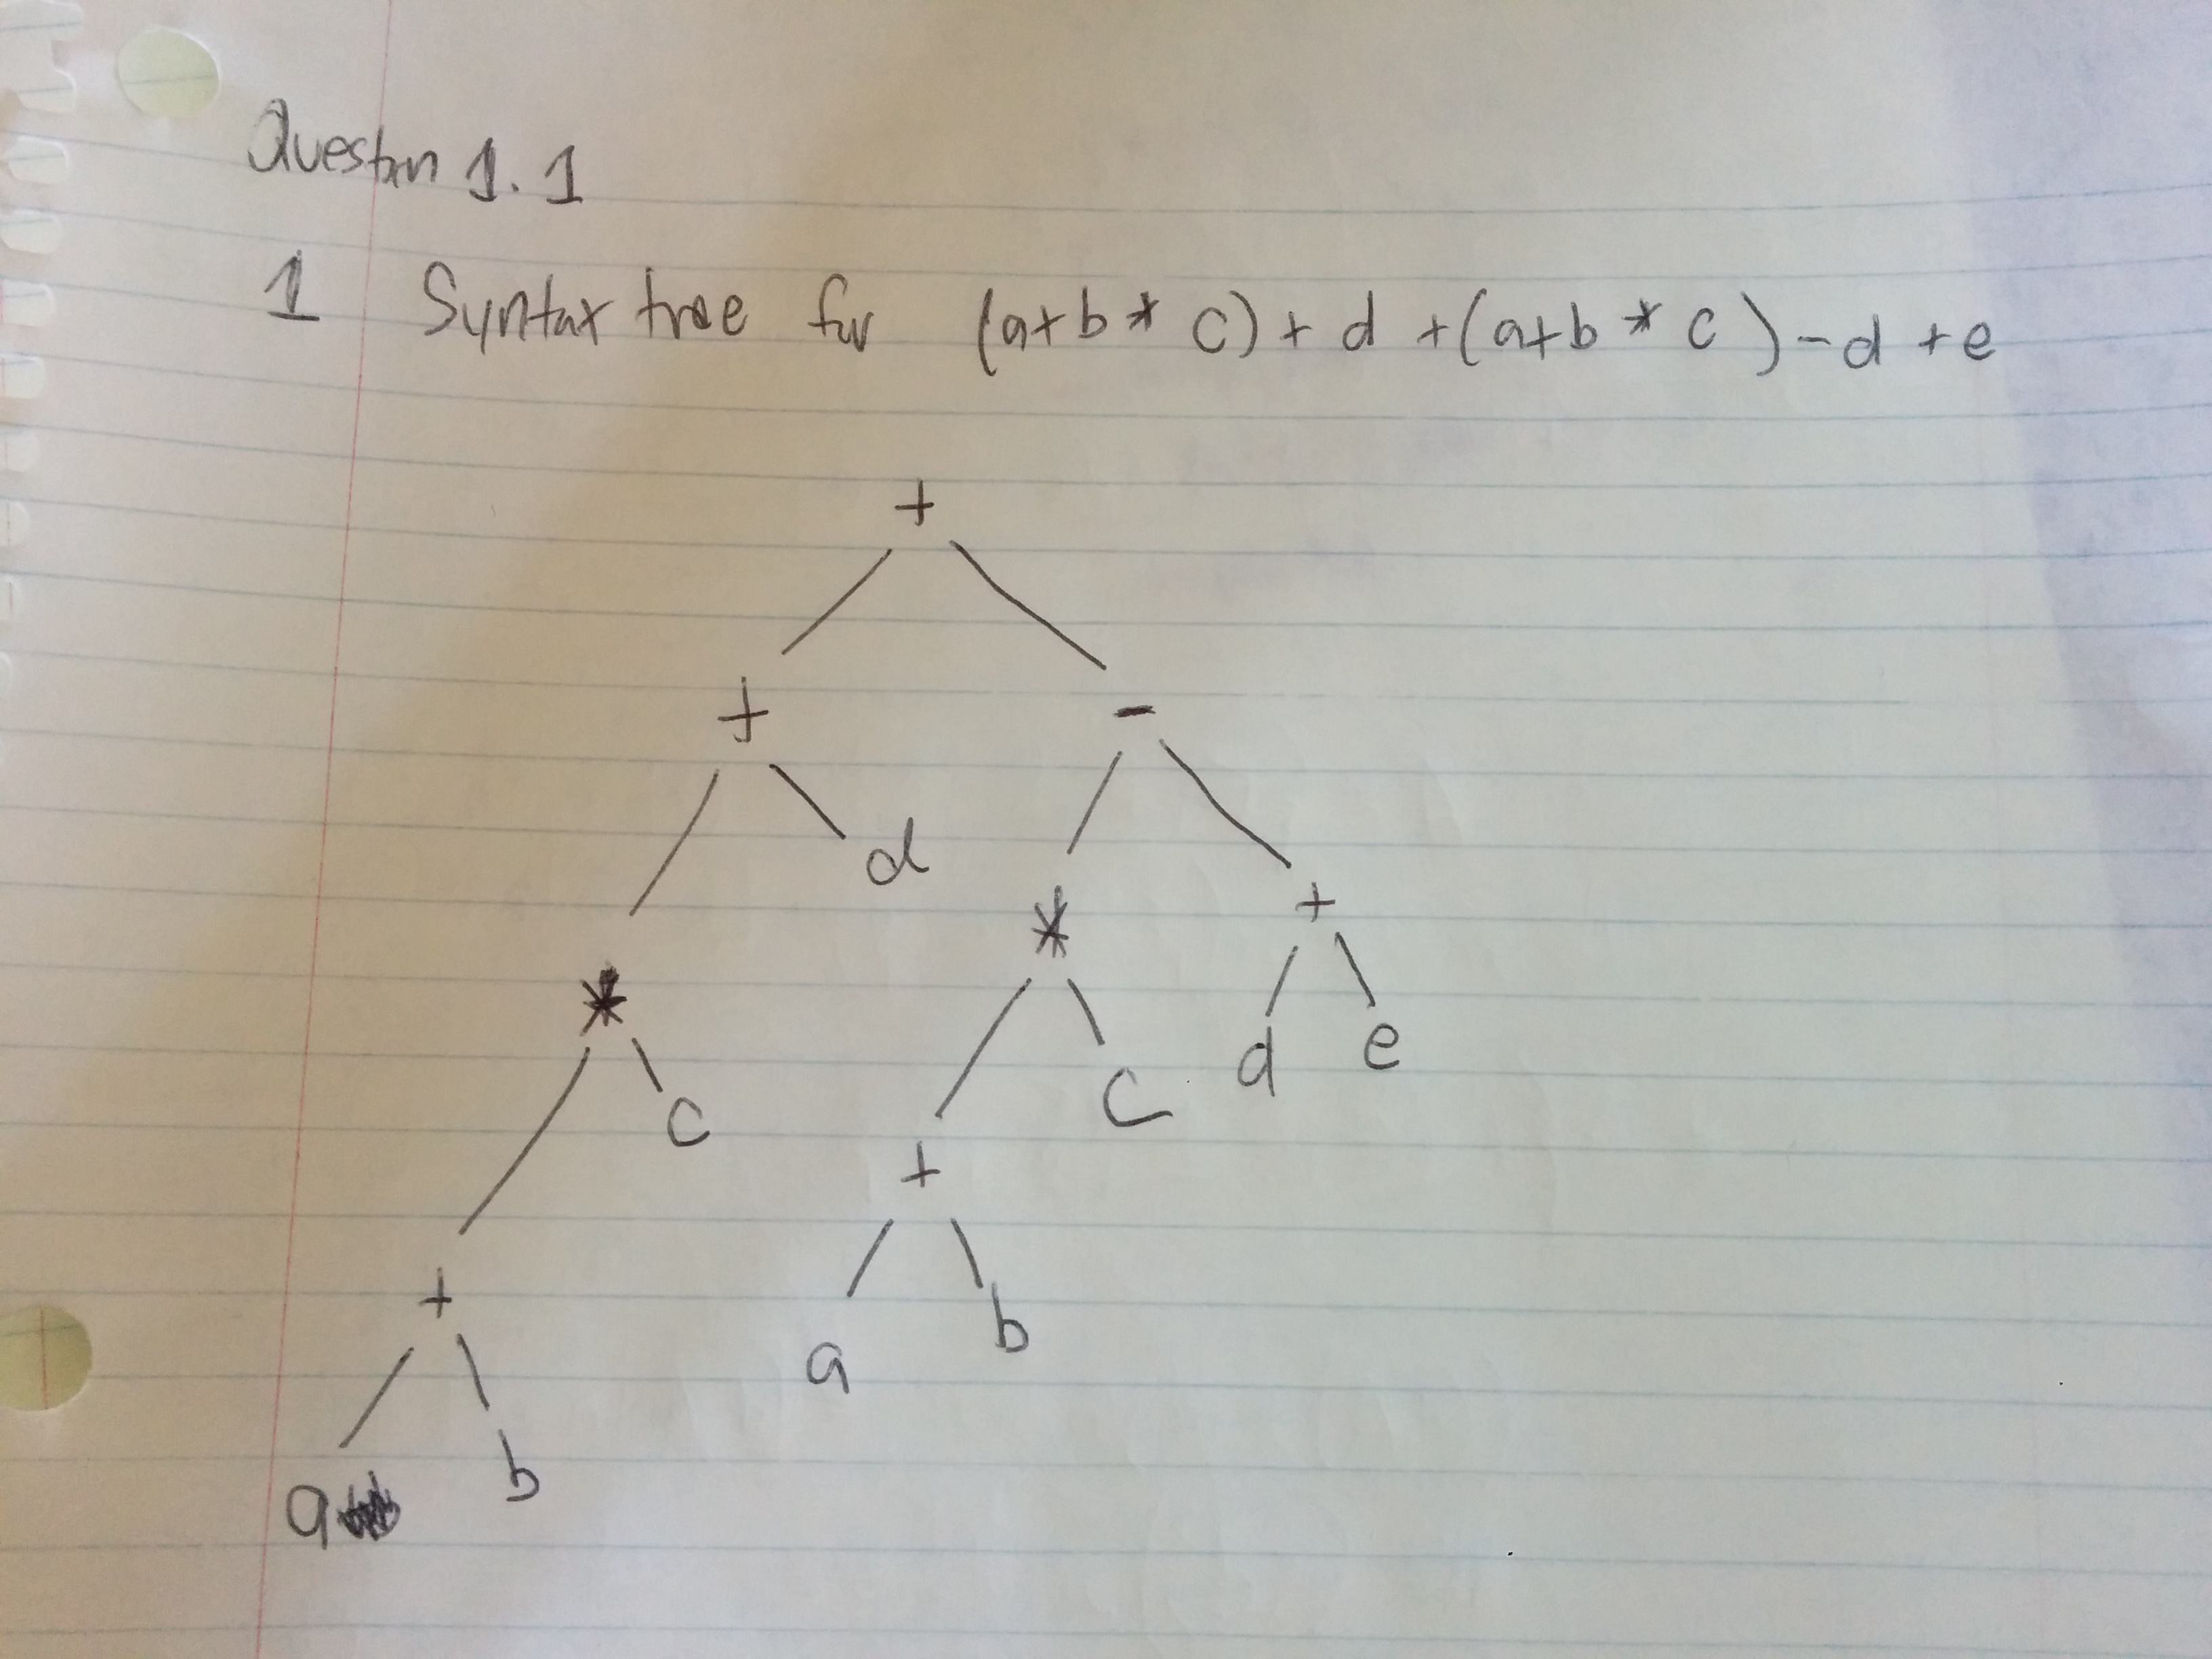
\includegraphics[scale=0.15]{IMG_20141025_154037.jpg}

\subsubsection{DAG (Directed Acyclic Graph) representation}
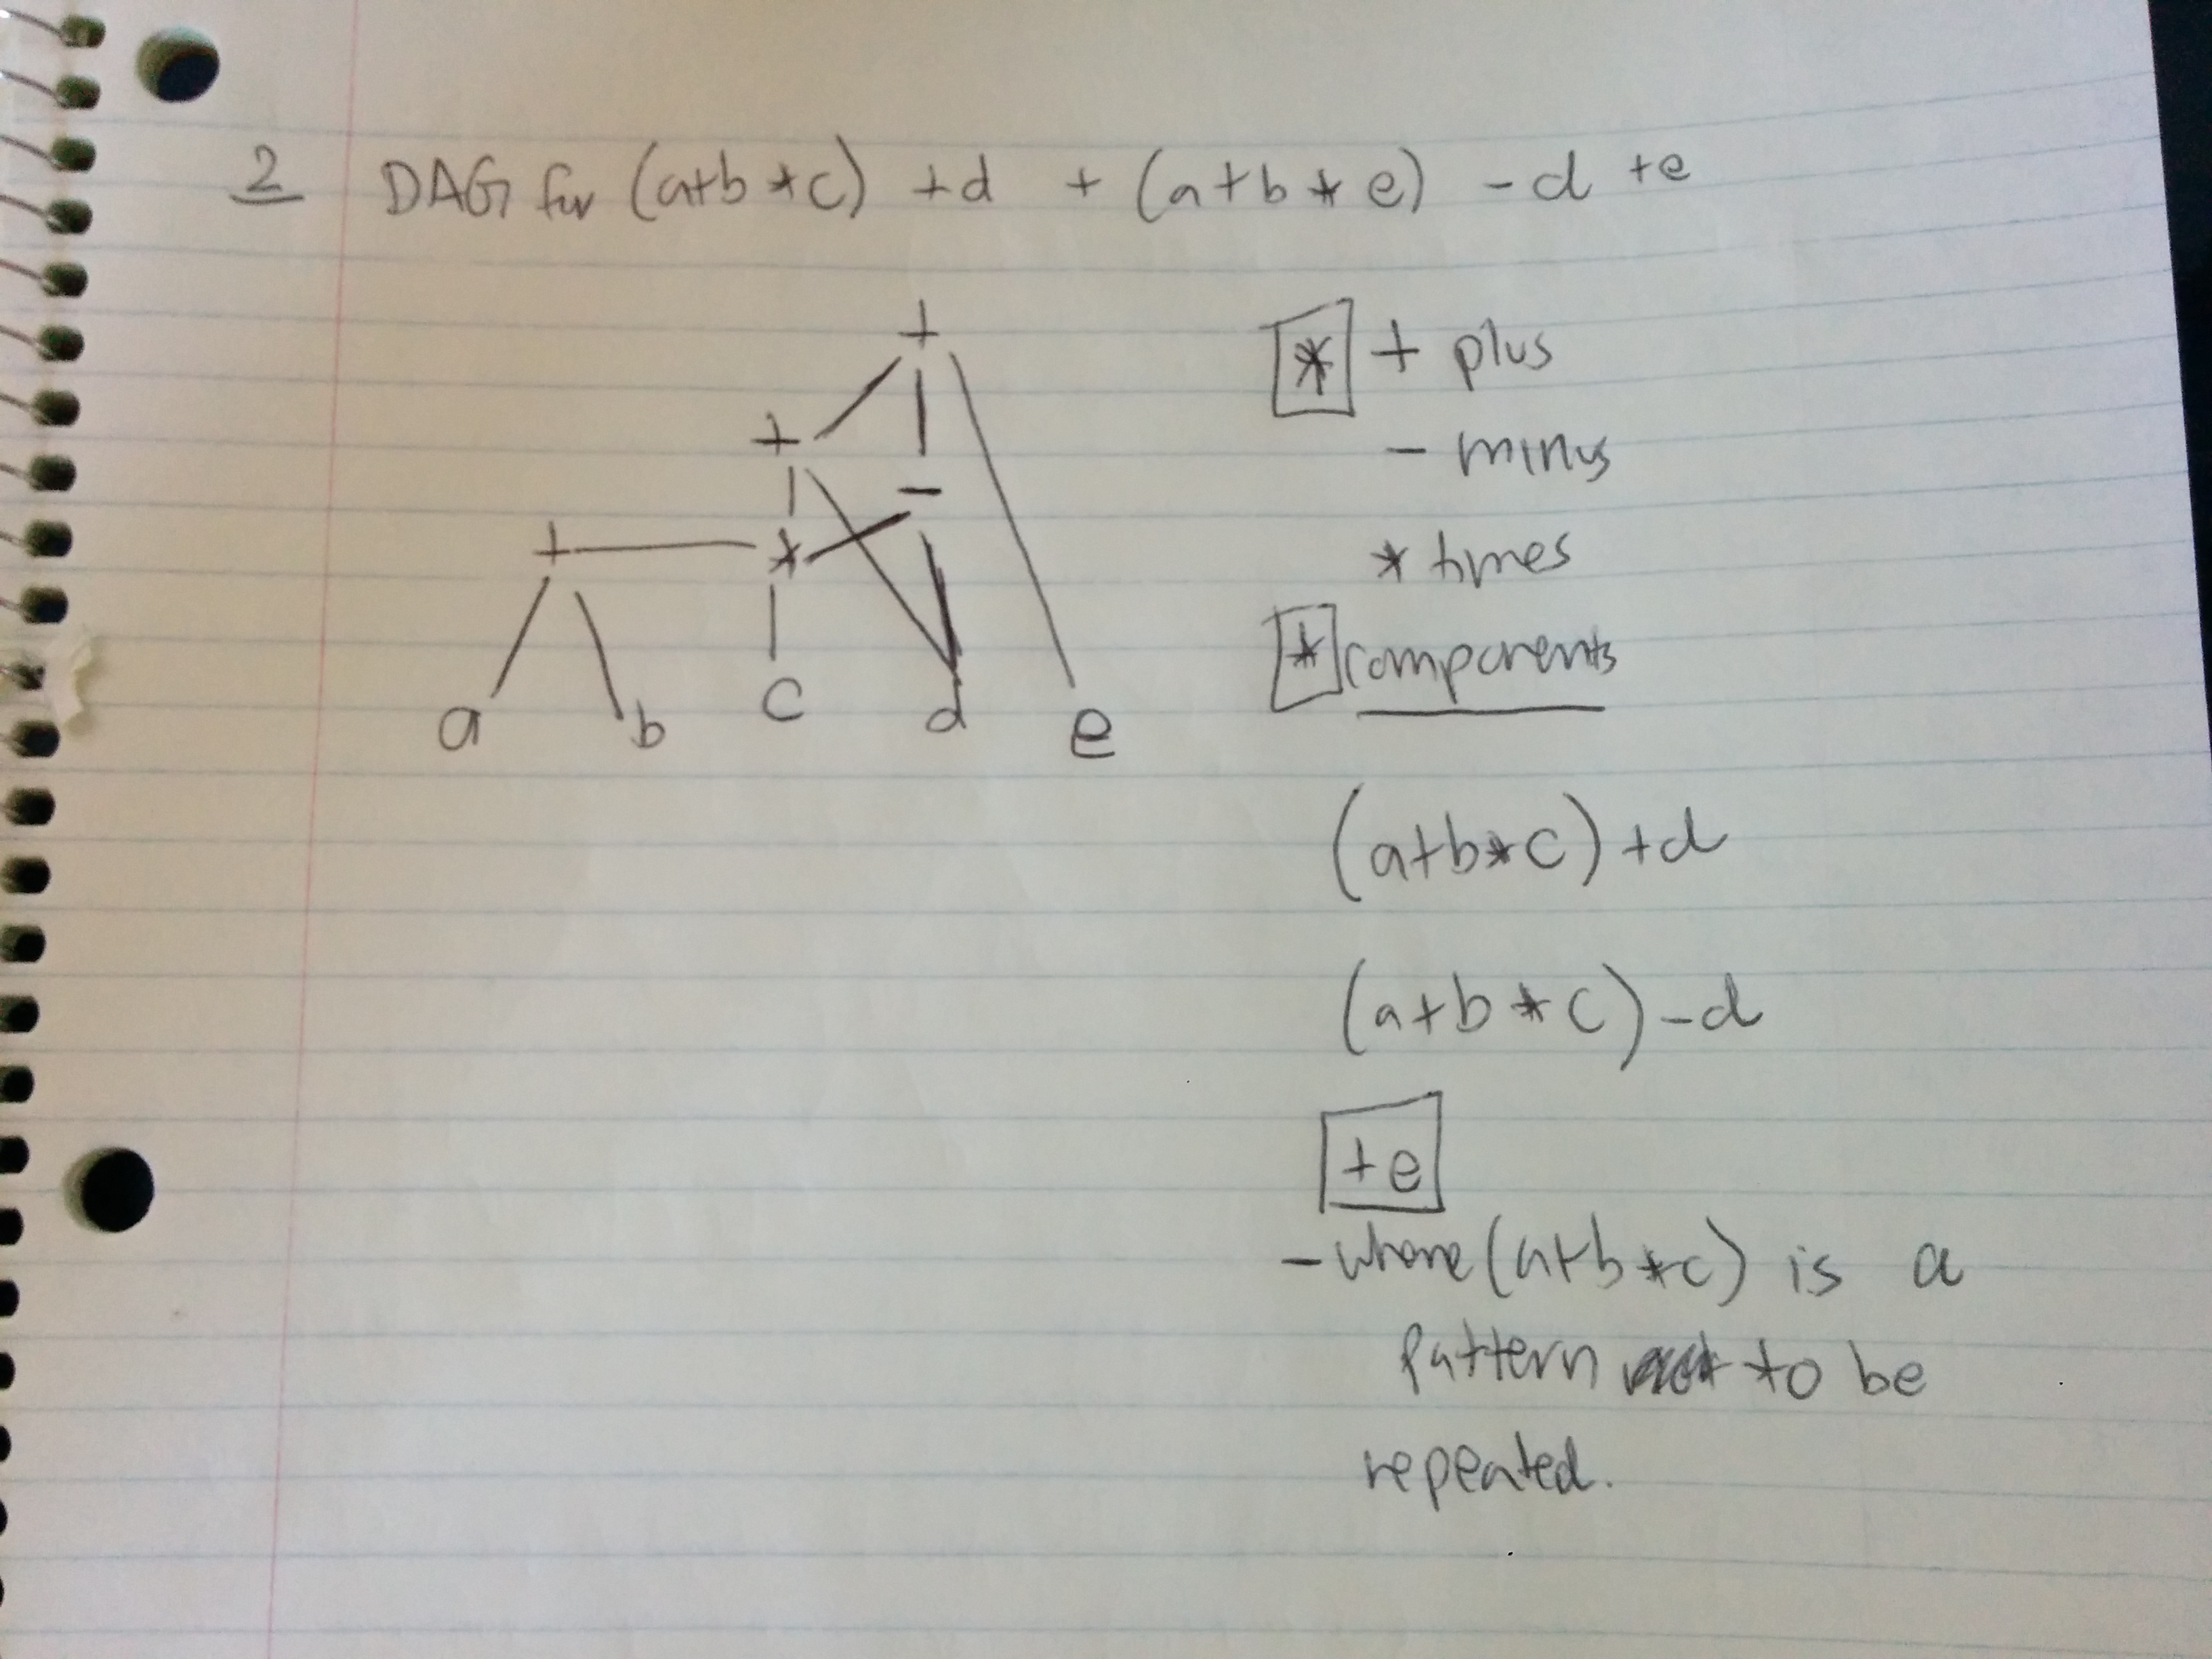
\includegraphics[scale=0.15]{IMG_20141025_154052.jpg}

\subsubsection{Three-Address Code representation}
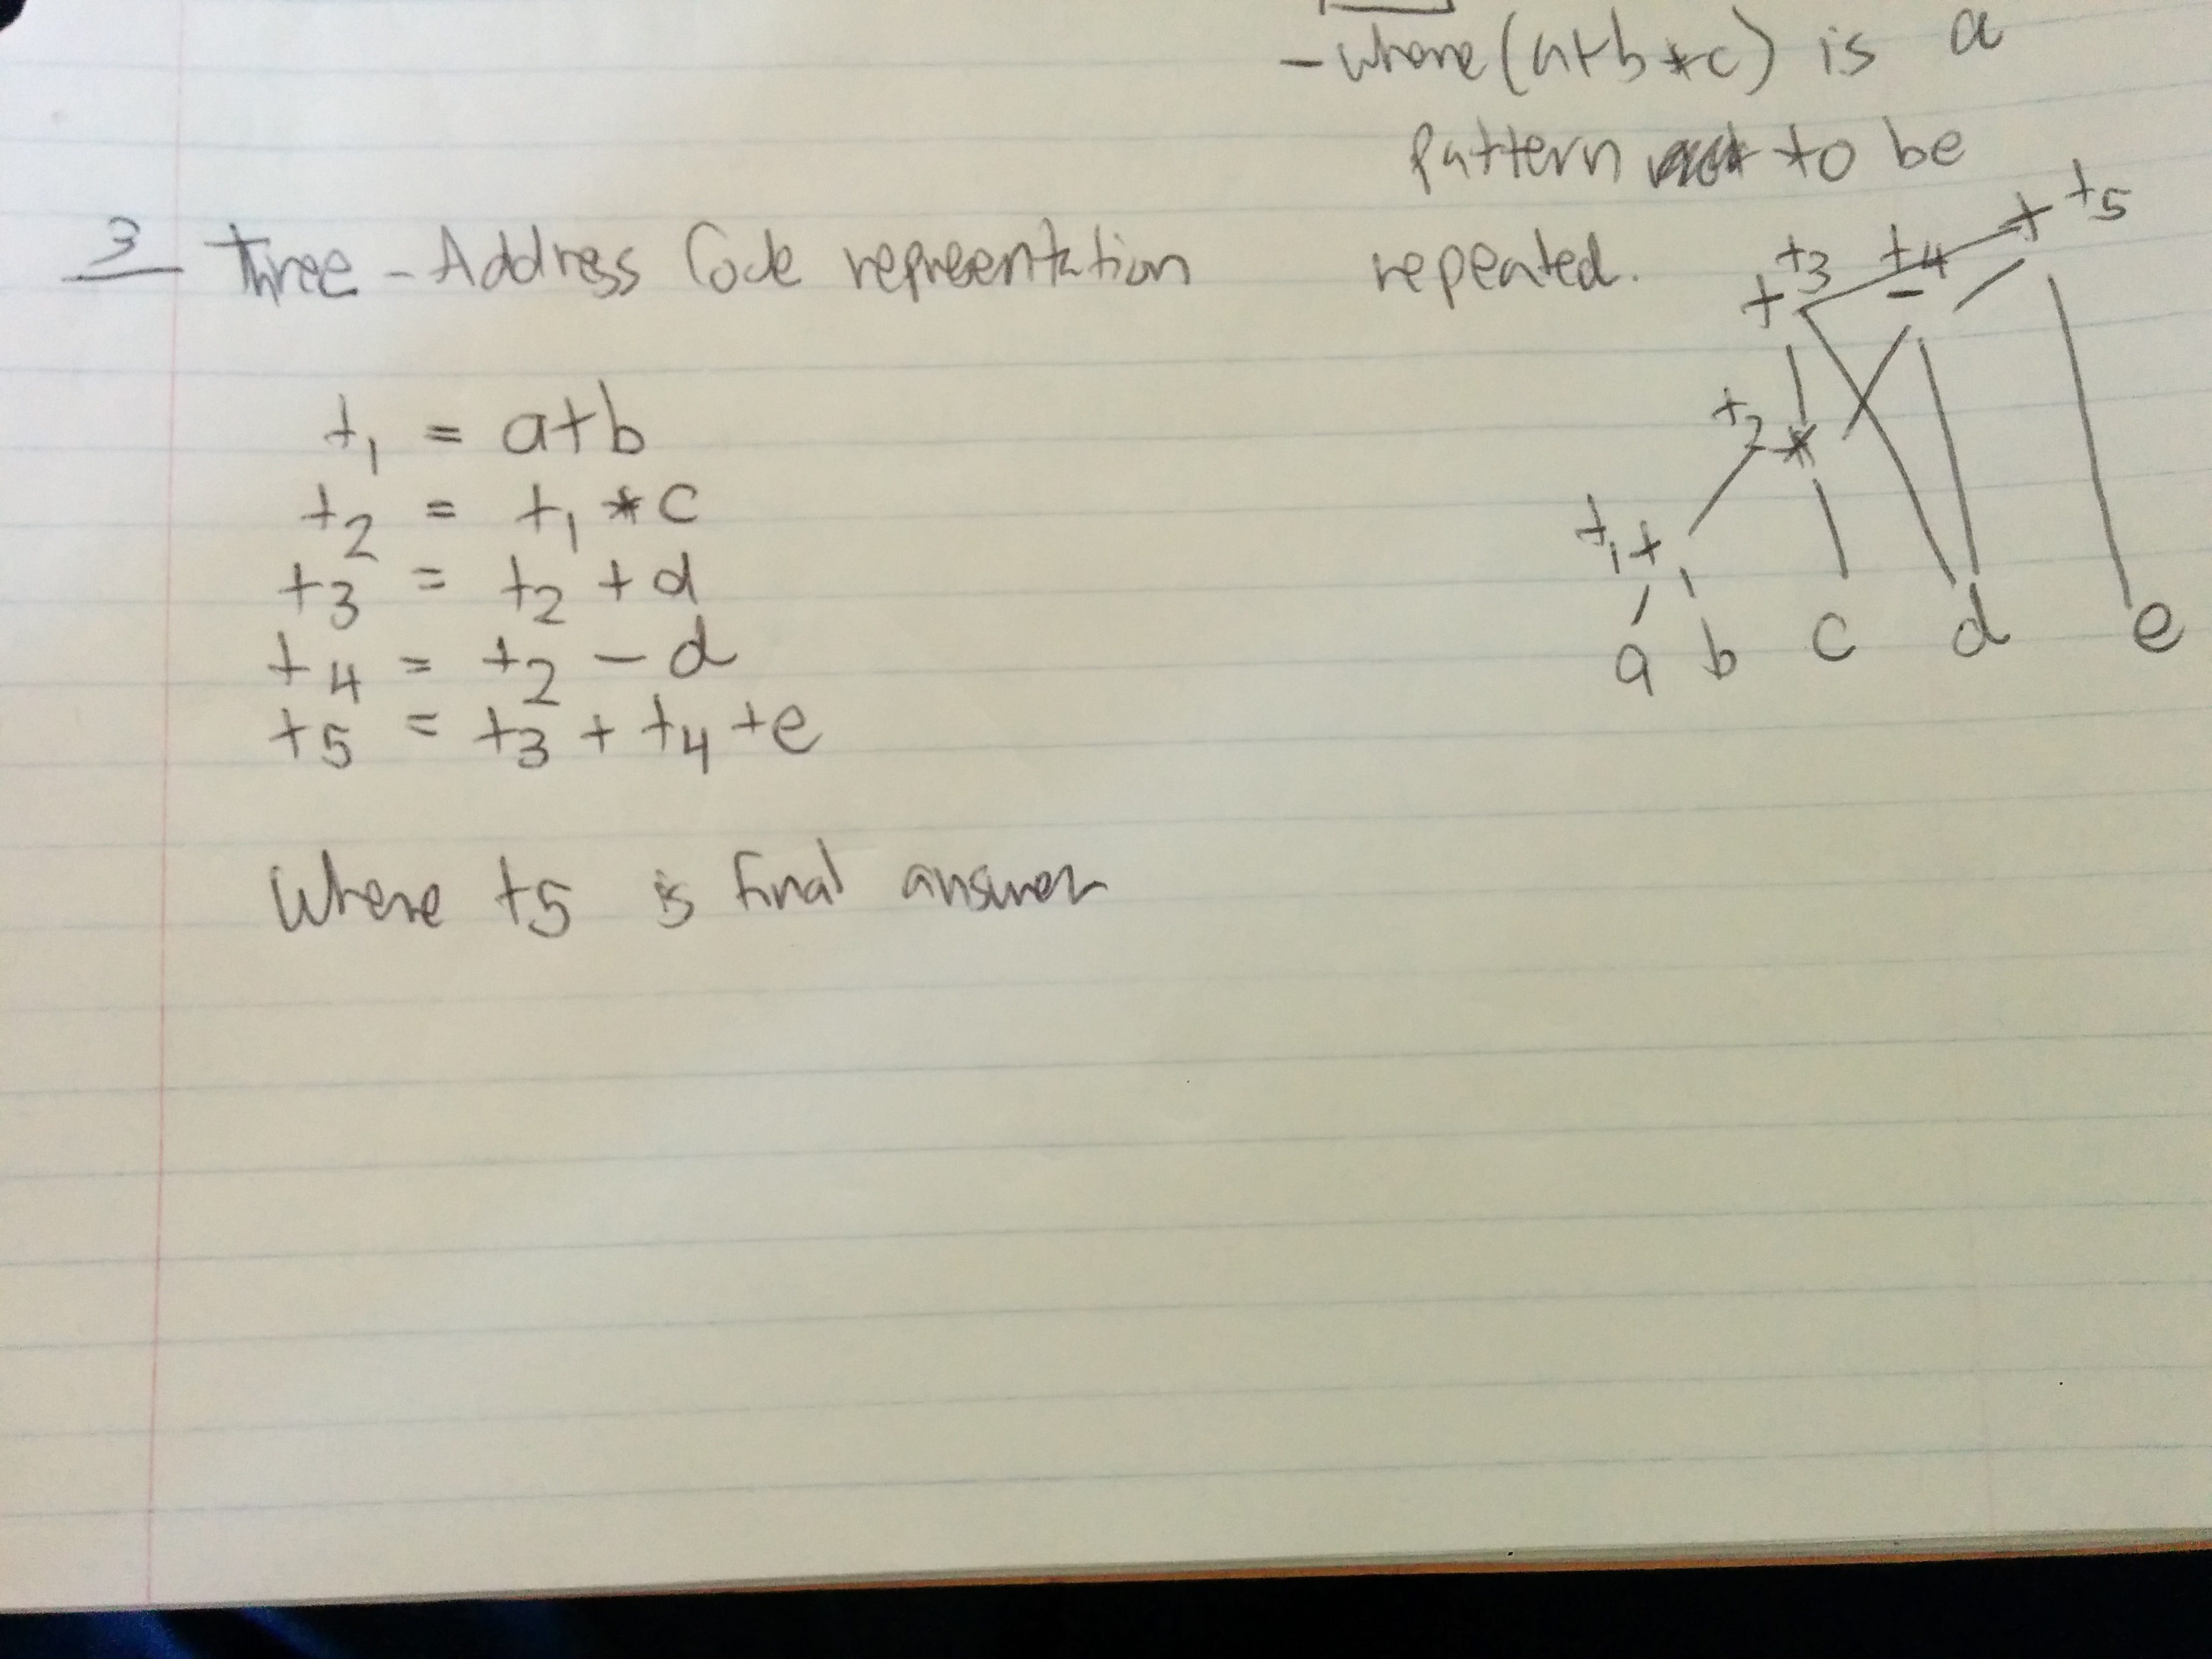
\includegraphics[scale=0.15]{IMG_20141025_154609.jpg}

\subsection{Question 1.2}

\subsubsection{Syntax Tree}
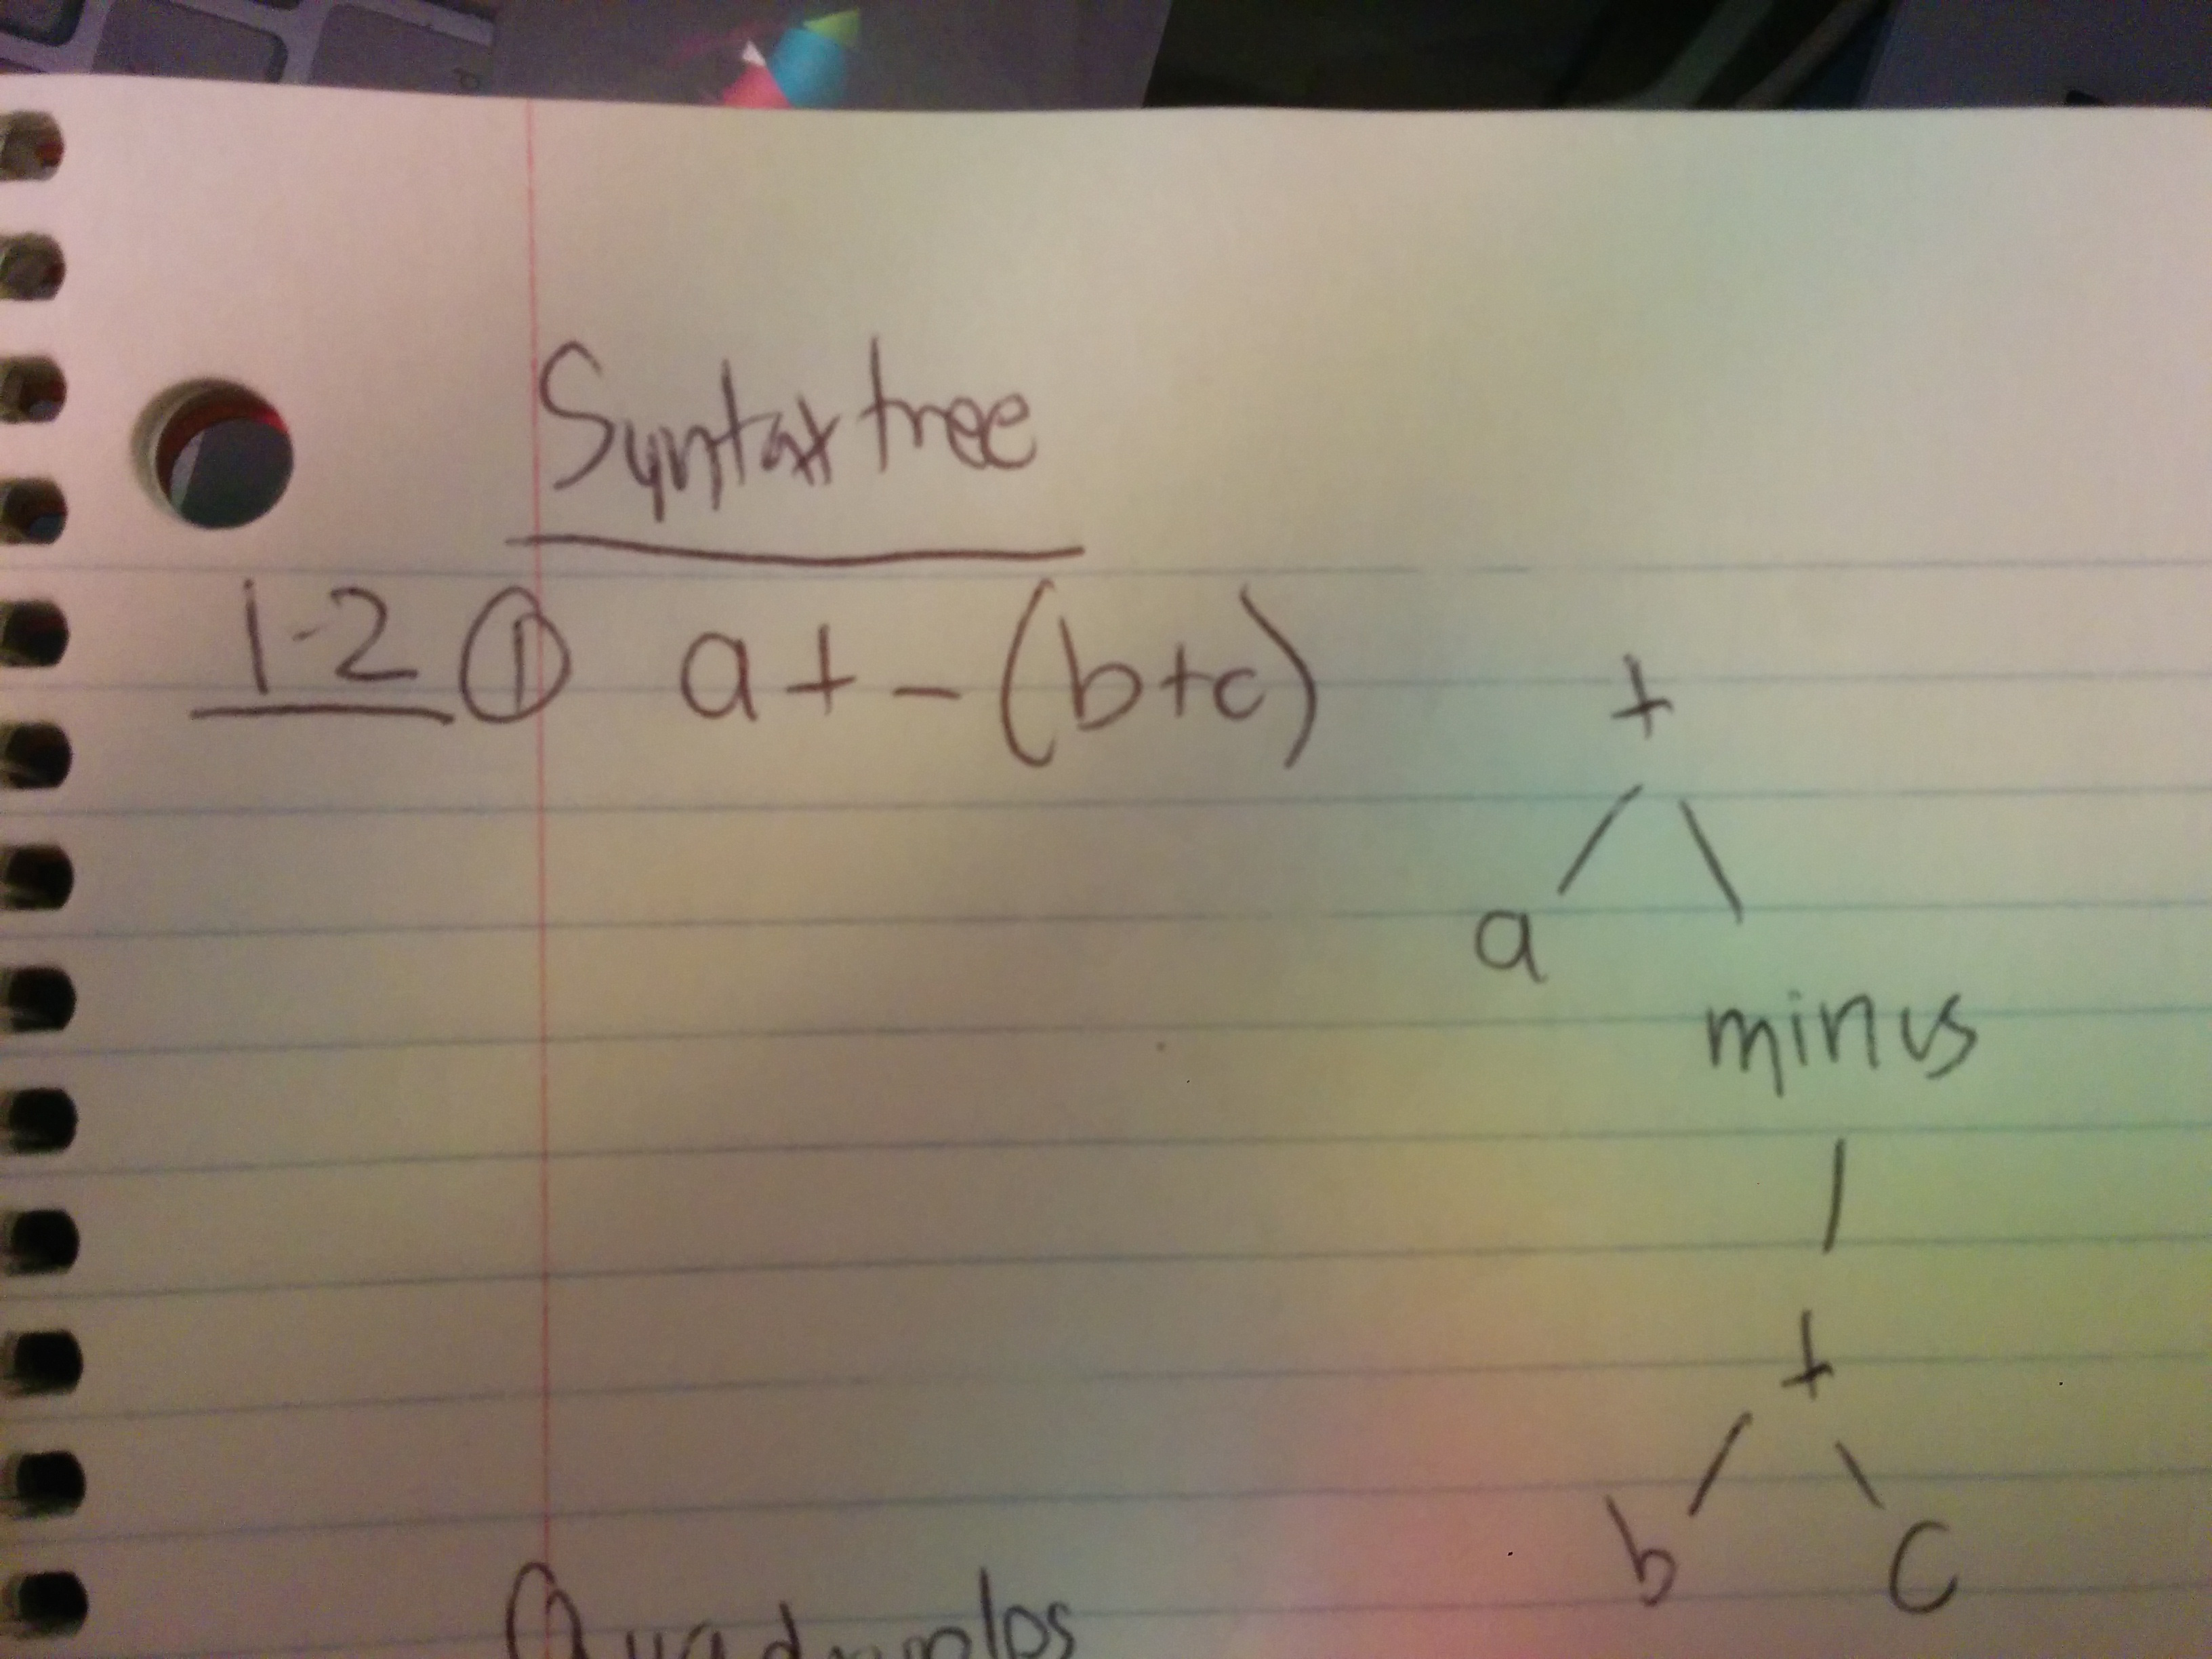
\includegraphics[scale=0.15]{IMG_20141028_235513.jpg}

\subsubsection{Quadruples}
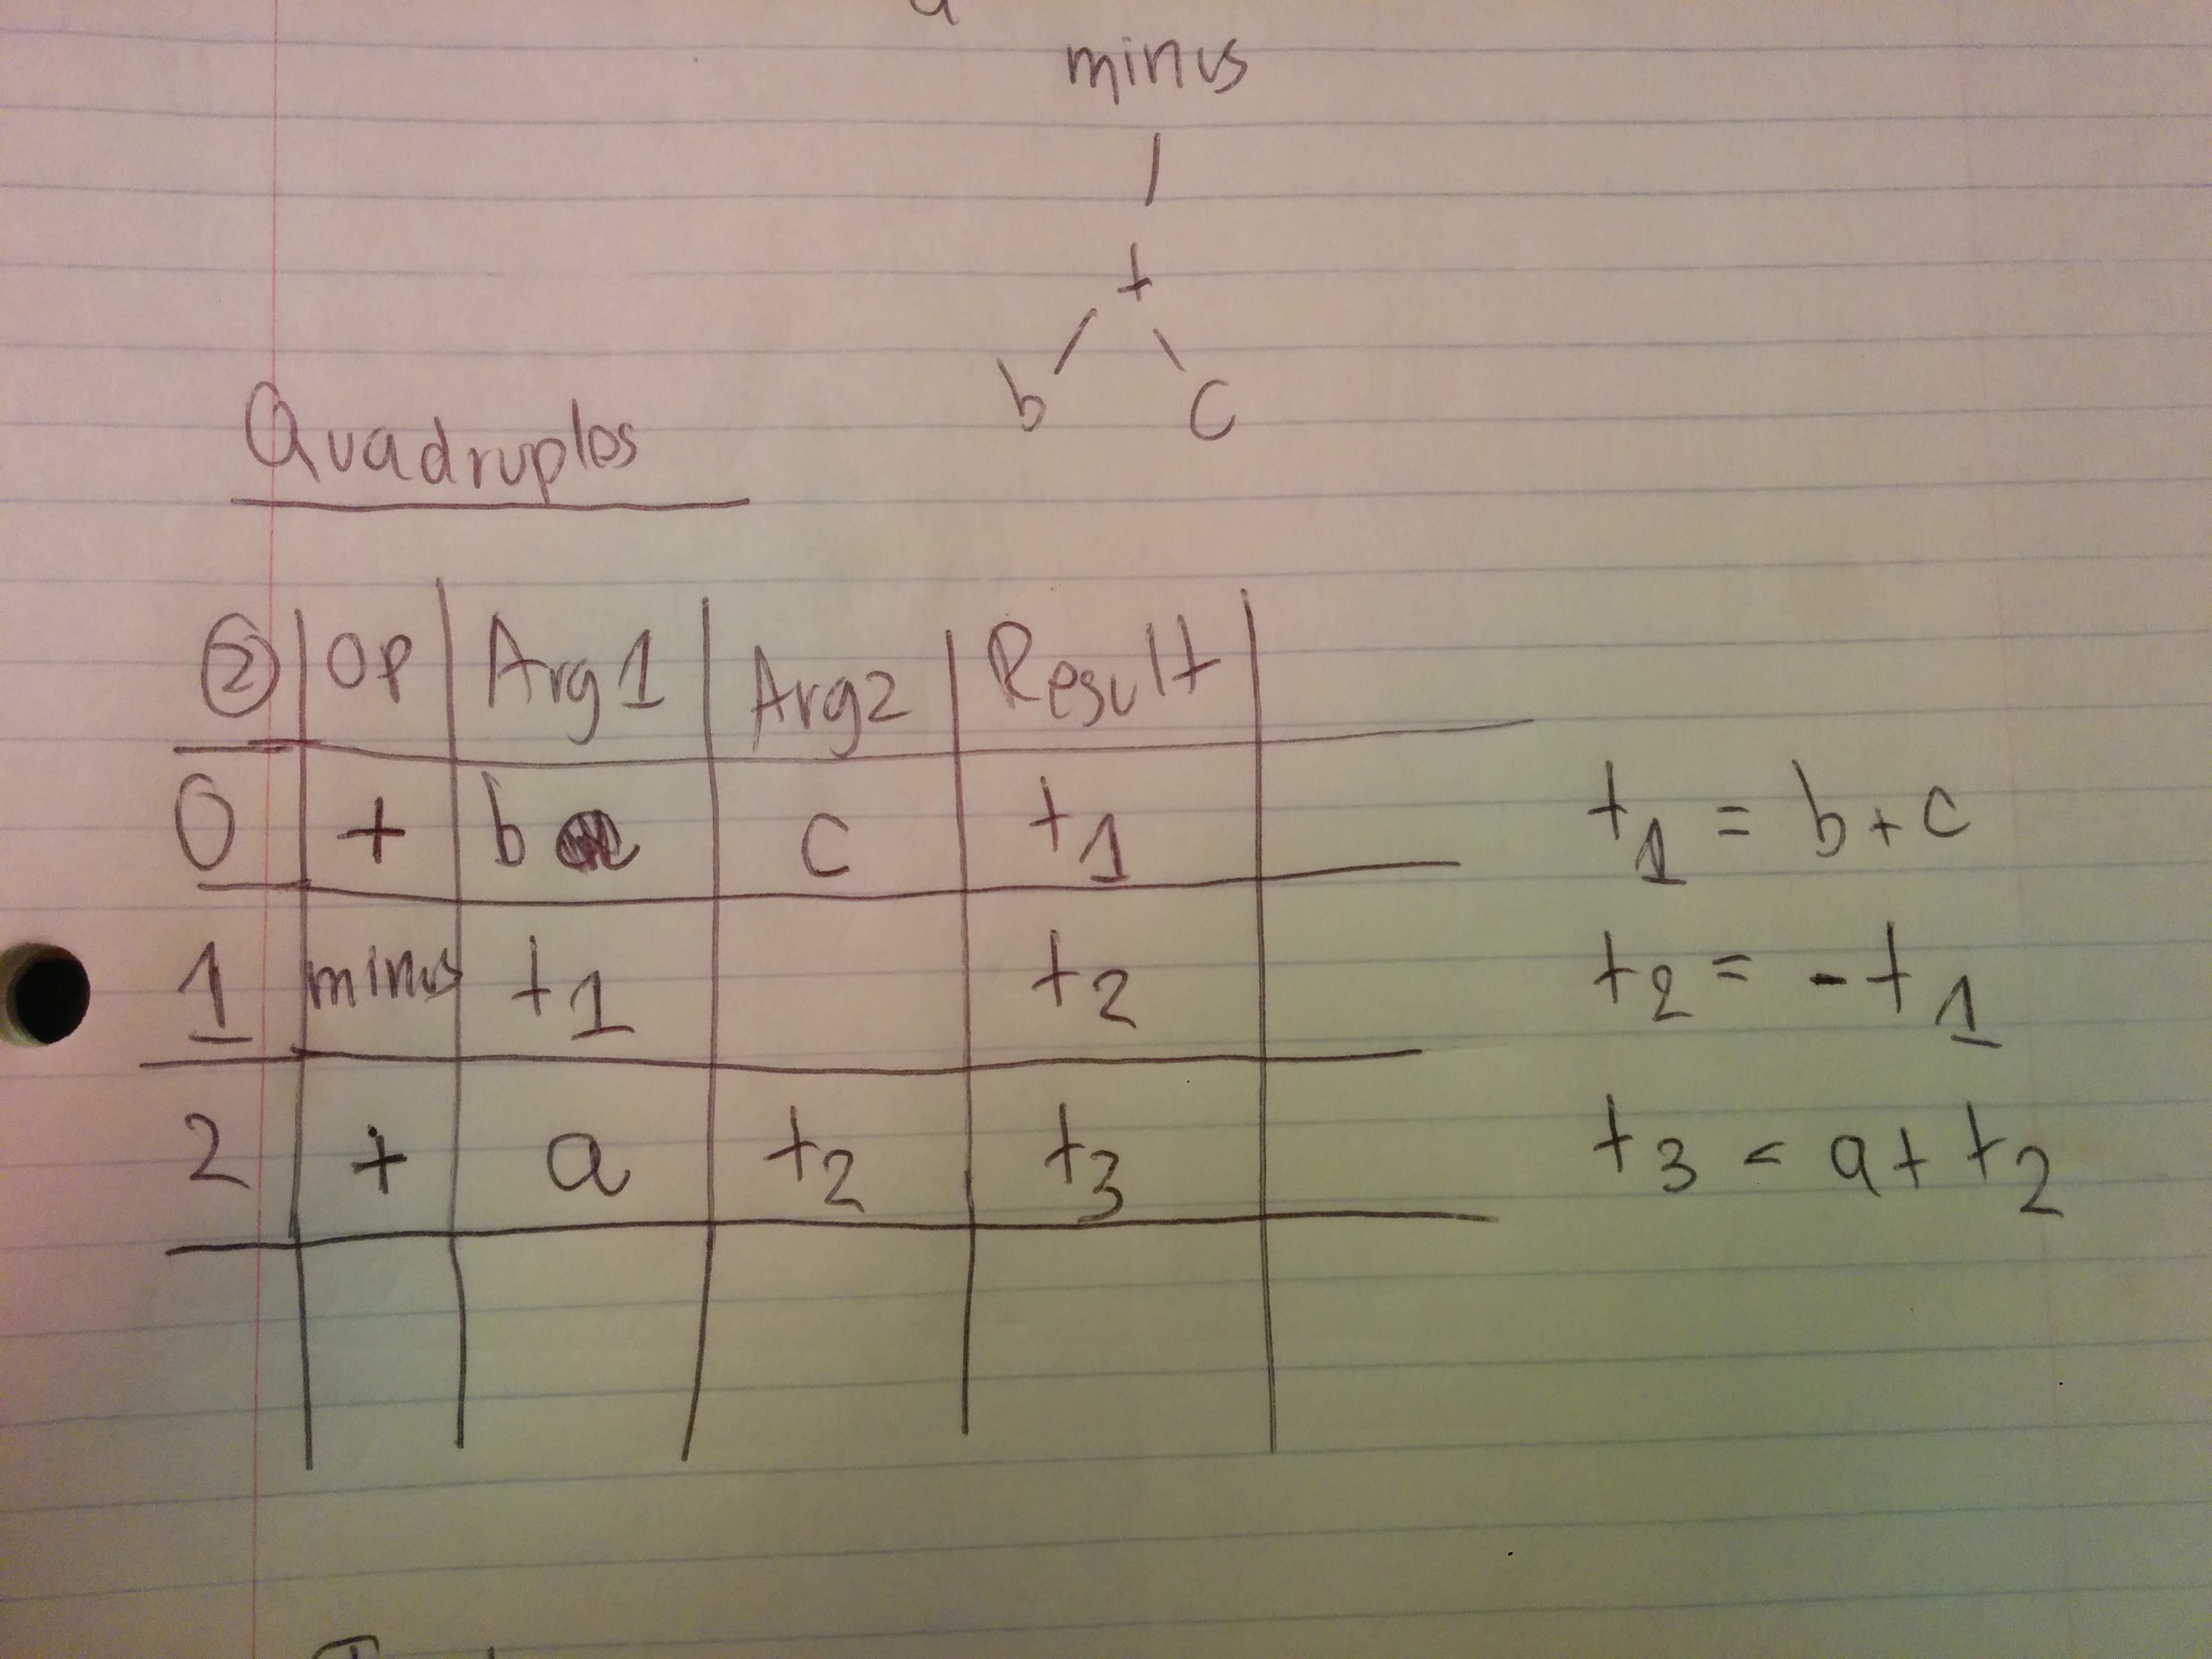
\includegraphics[scale=0.15]{IMG_20141028_235505.jpg}

\subsubsection{Triples}
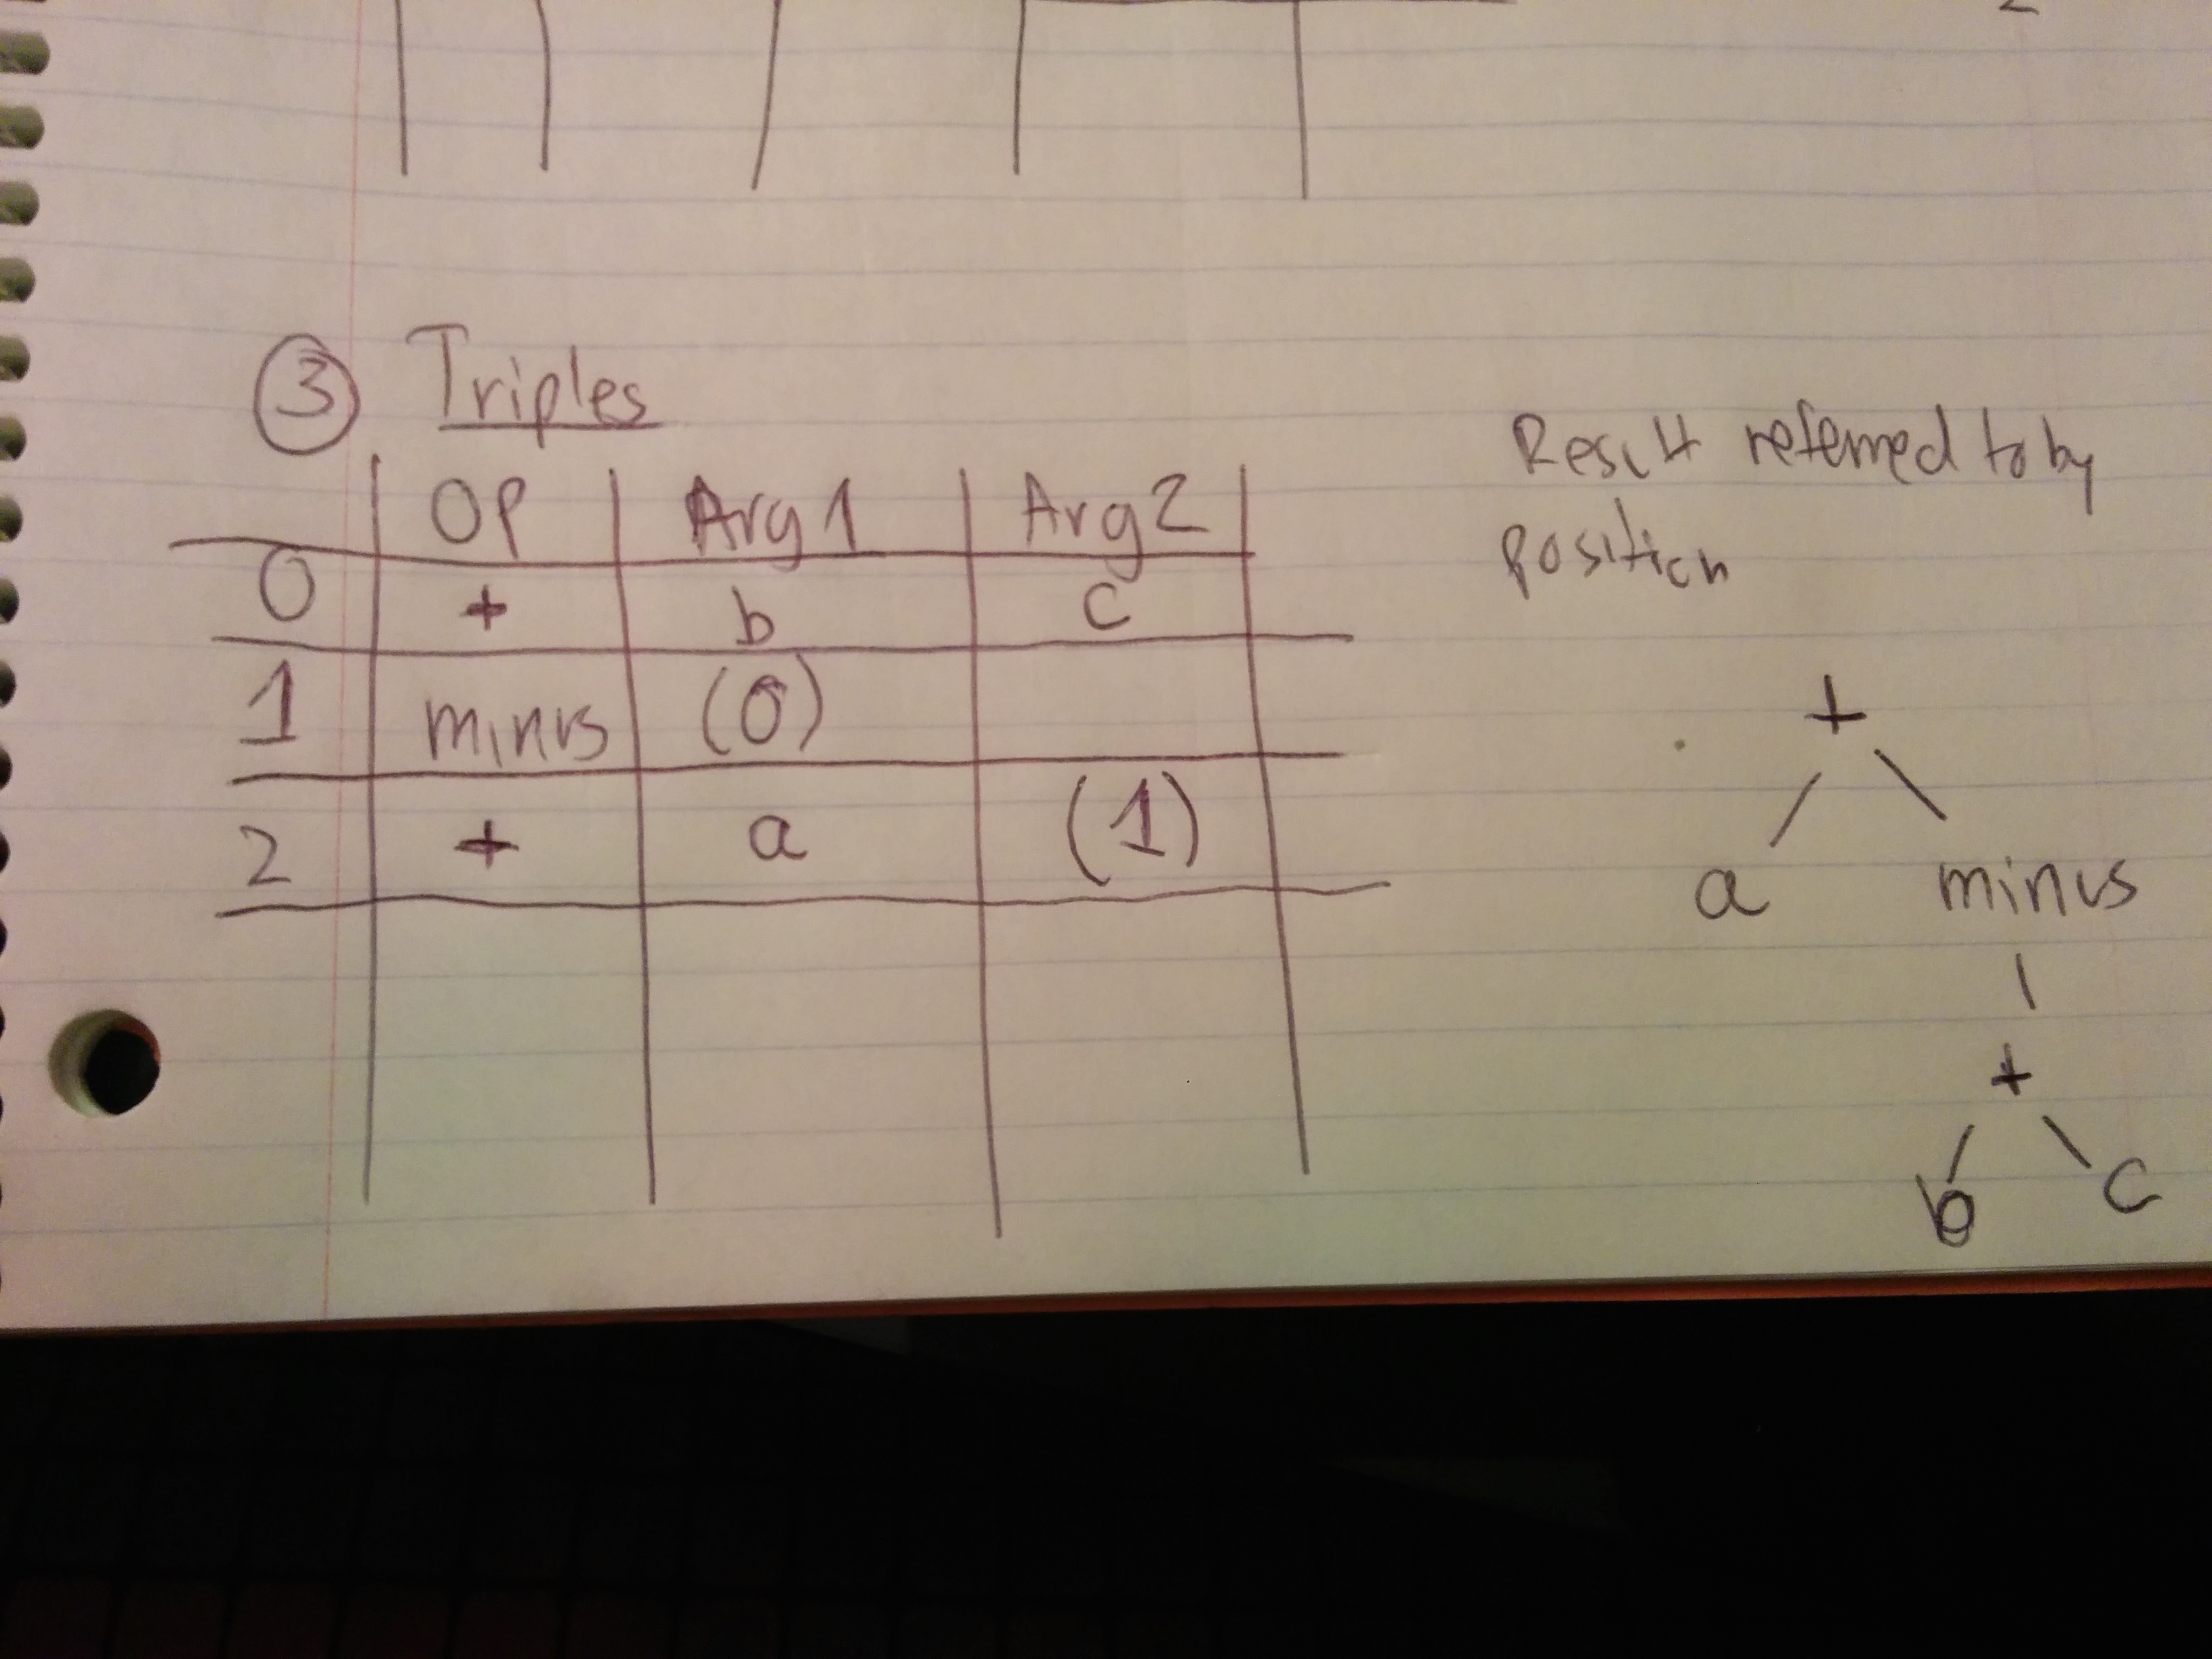
\includegraphics[scale=0.15]{IMG_20141028_235519.jpg}

\subsubsection{Indirect Triples}
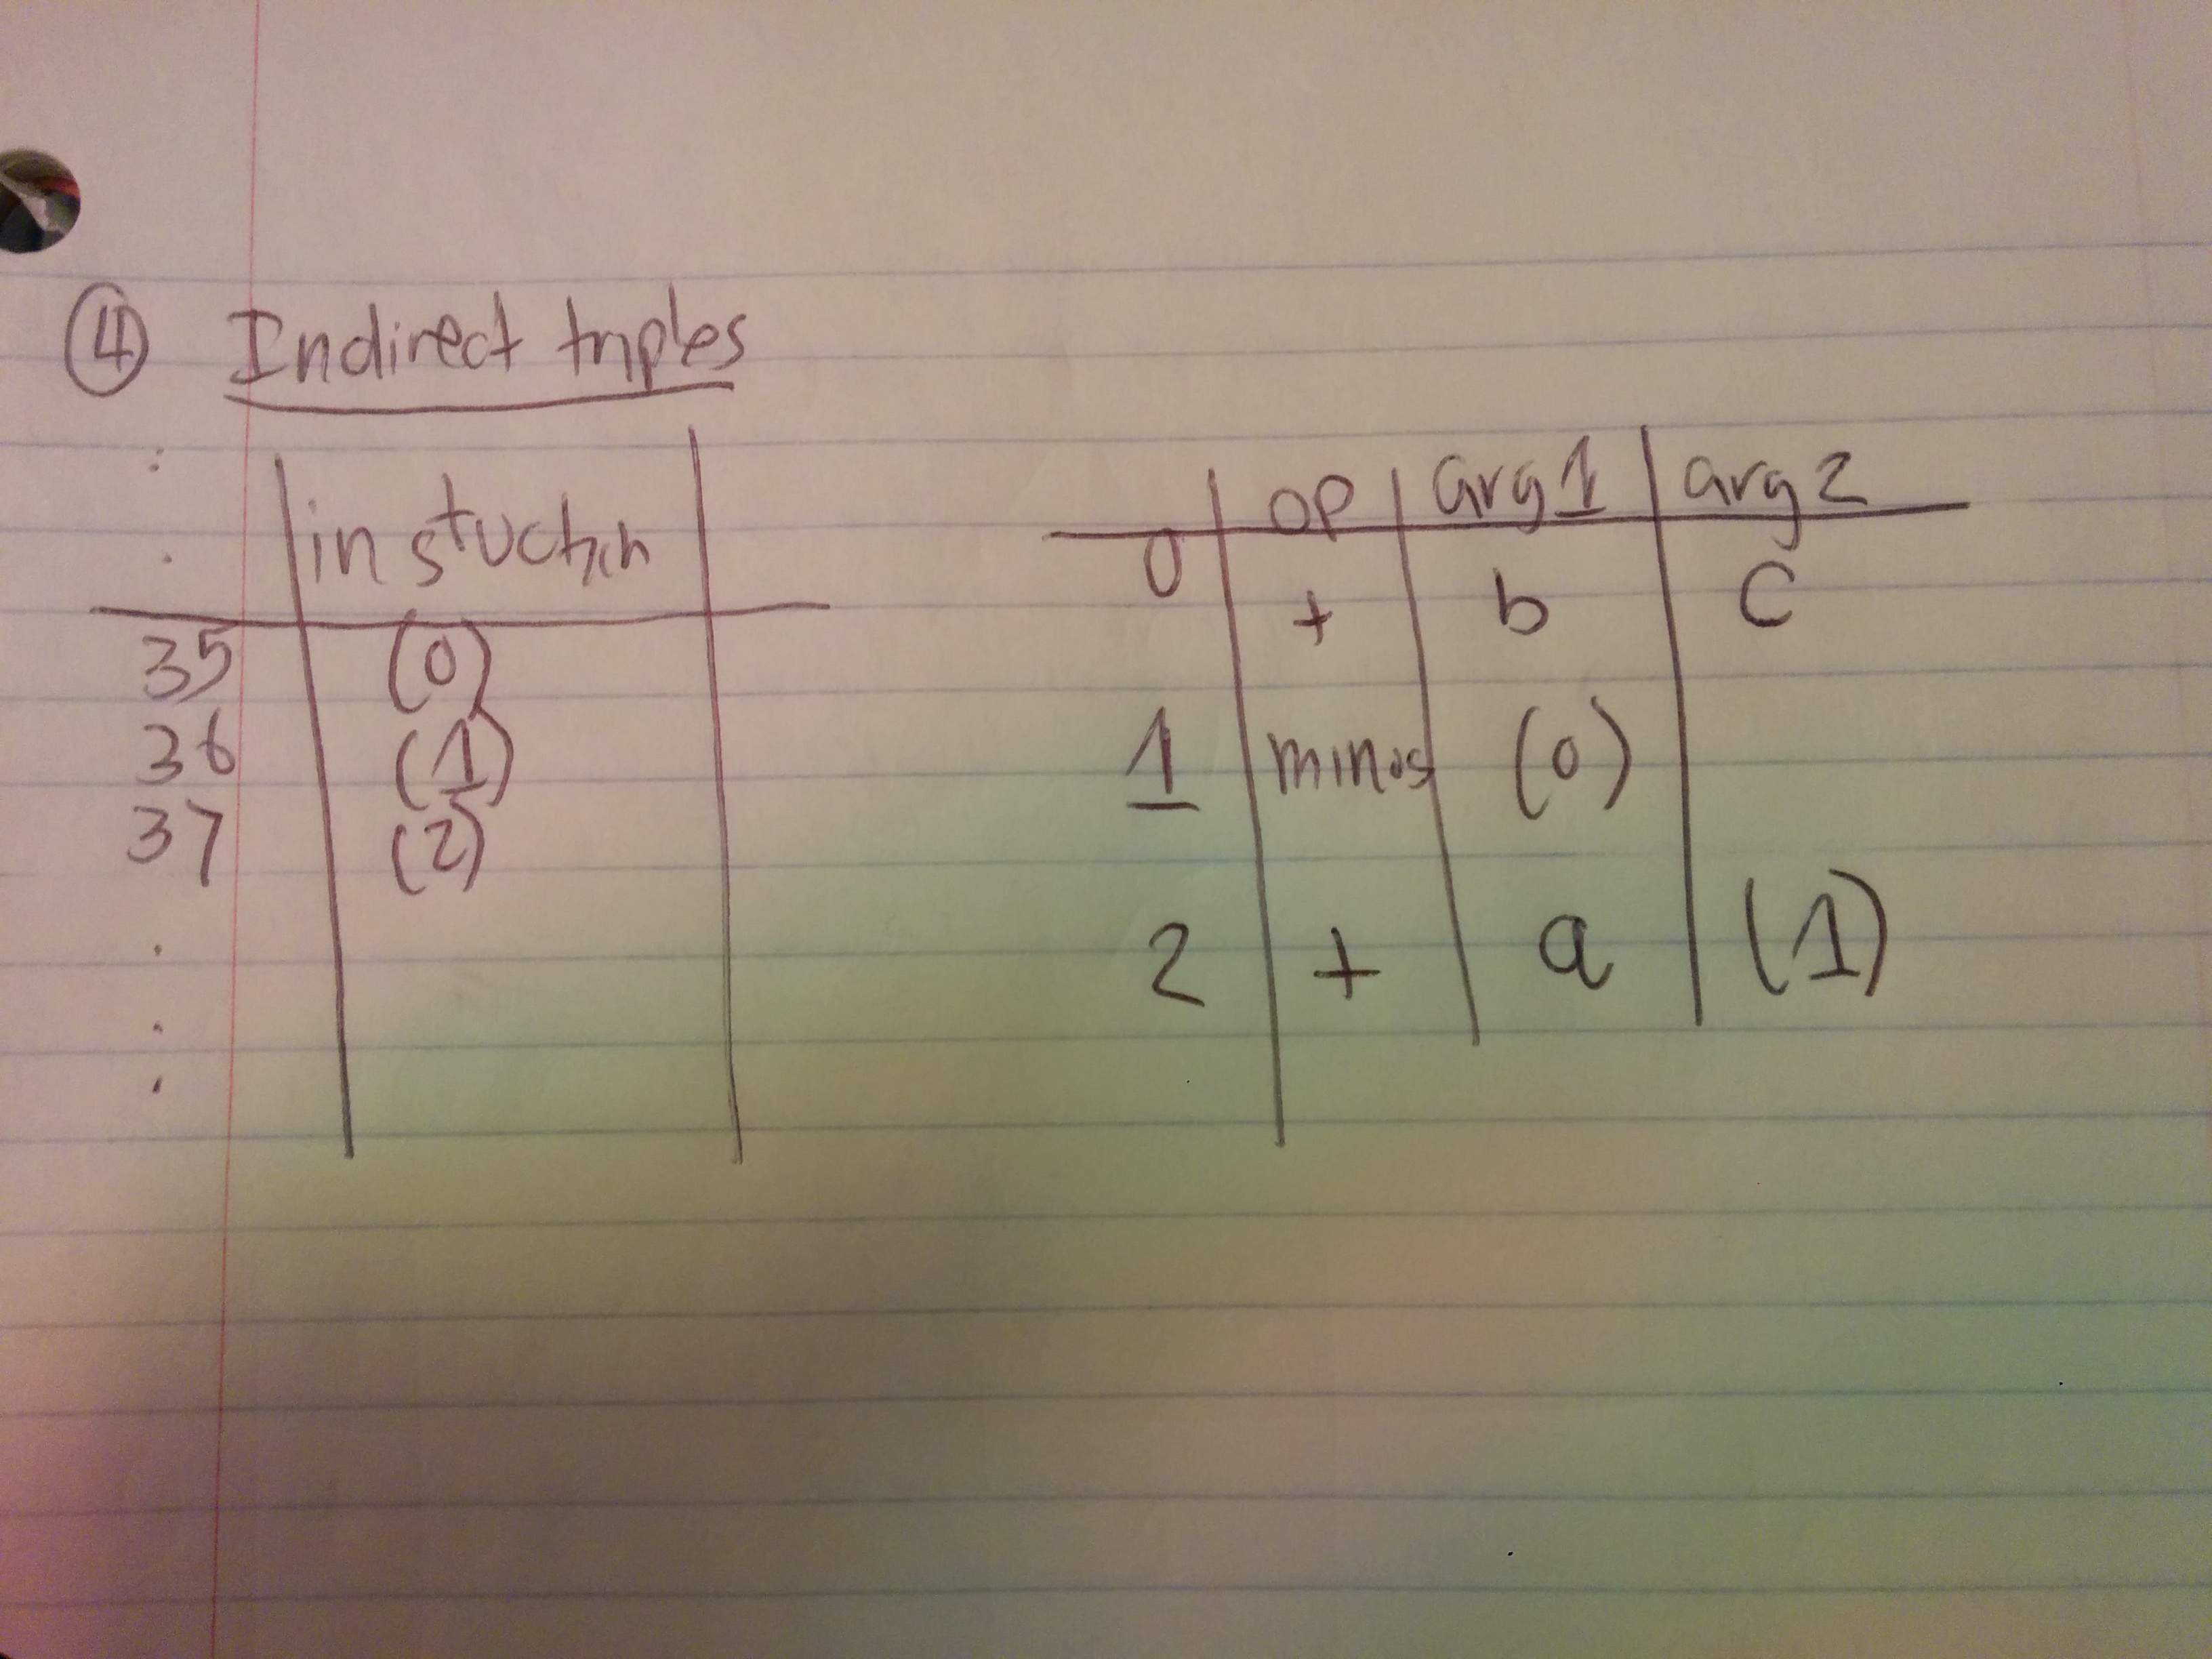
\includegraphics[scale=0.15]{IMG_20141029_001005.jpg}

\newpage

\section{Translation}

\subsection{Question 2.1}

\subsubsection{Add a translation rule for the following expression production: \\ E $\rightarrow$ E1 * E2}
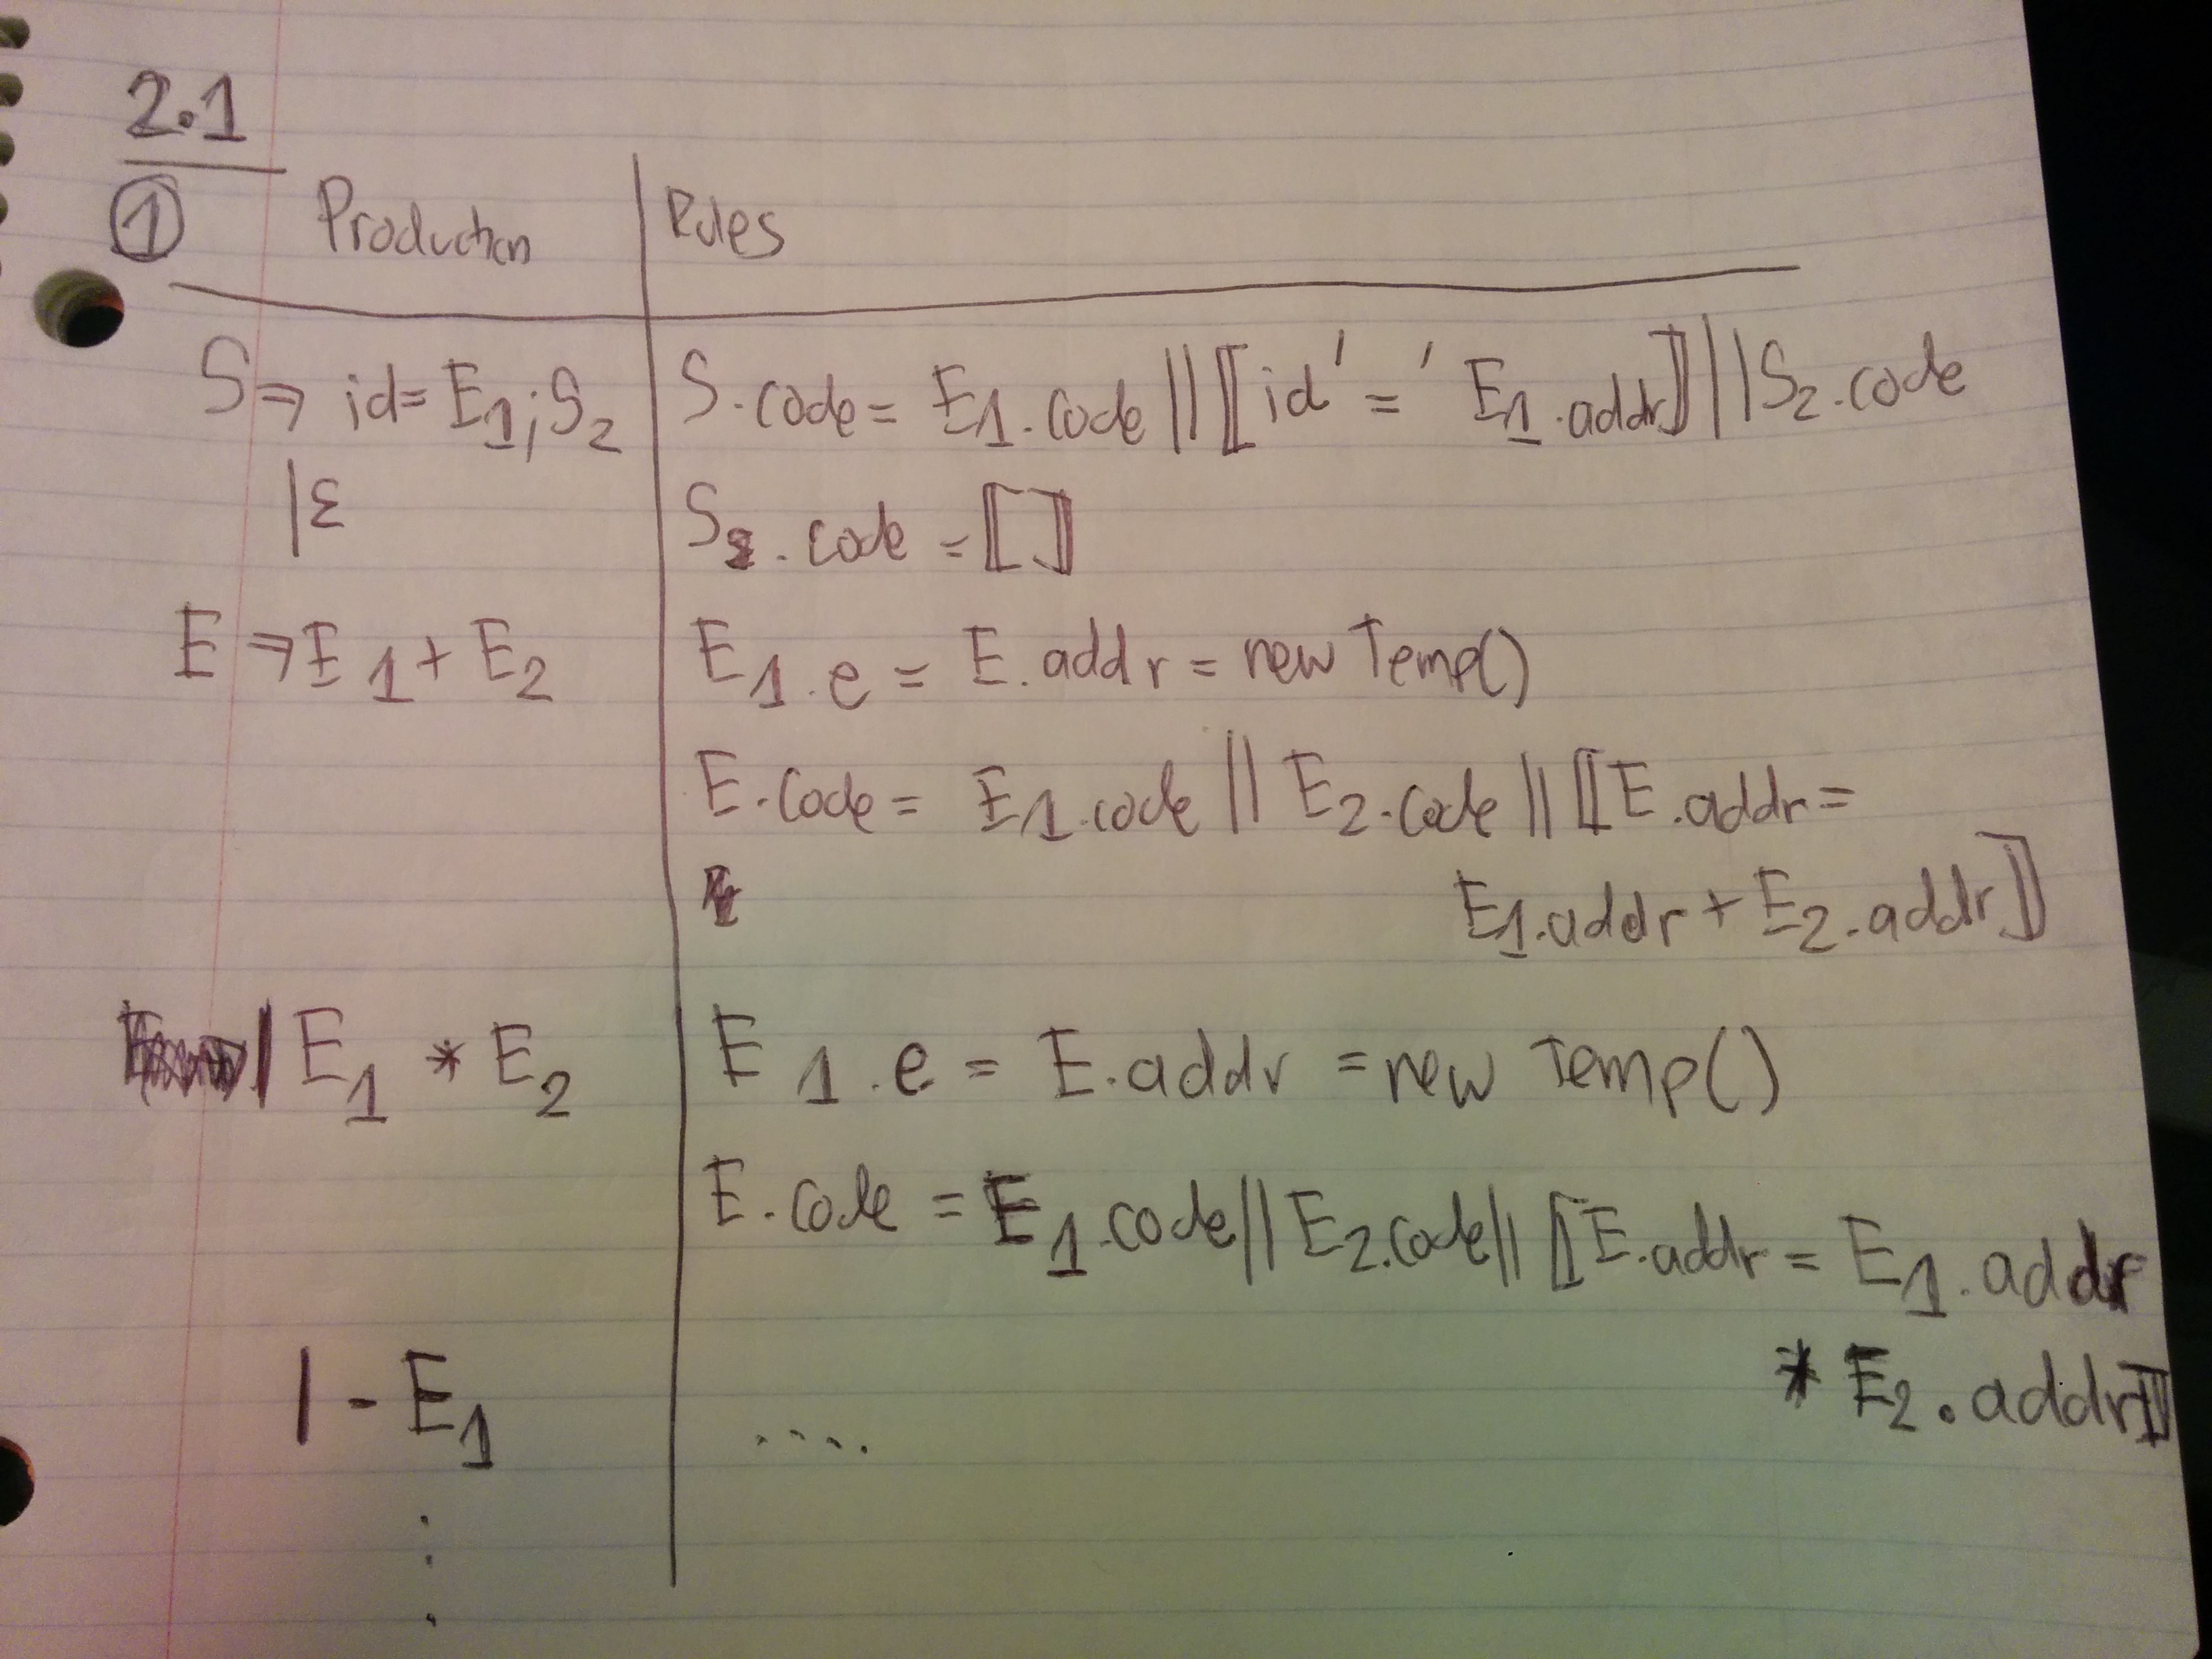
\includegraphics[scale=0.15]{IMG_20141029_003207.jpg}

\subsection{Question 2.2}
\subsubsection{Explain how the code is expected to evaluate, assuming parameters are passed call-by-value.}

\subsection{Question 2.3}
\subsubsection{S $\rightarrow$ for(S1; B; S2) S3 \\ Extending the code from the book}
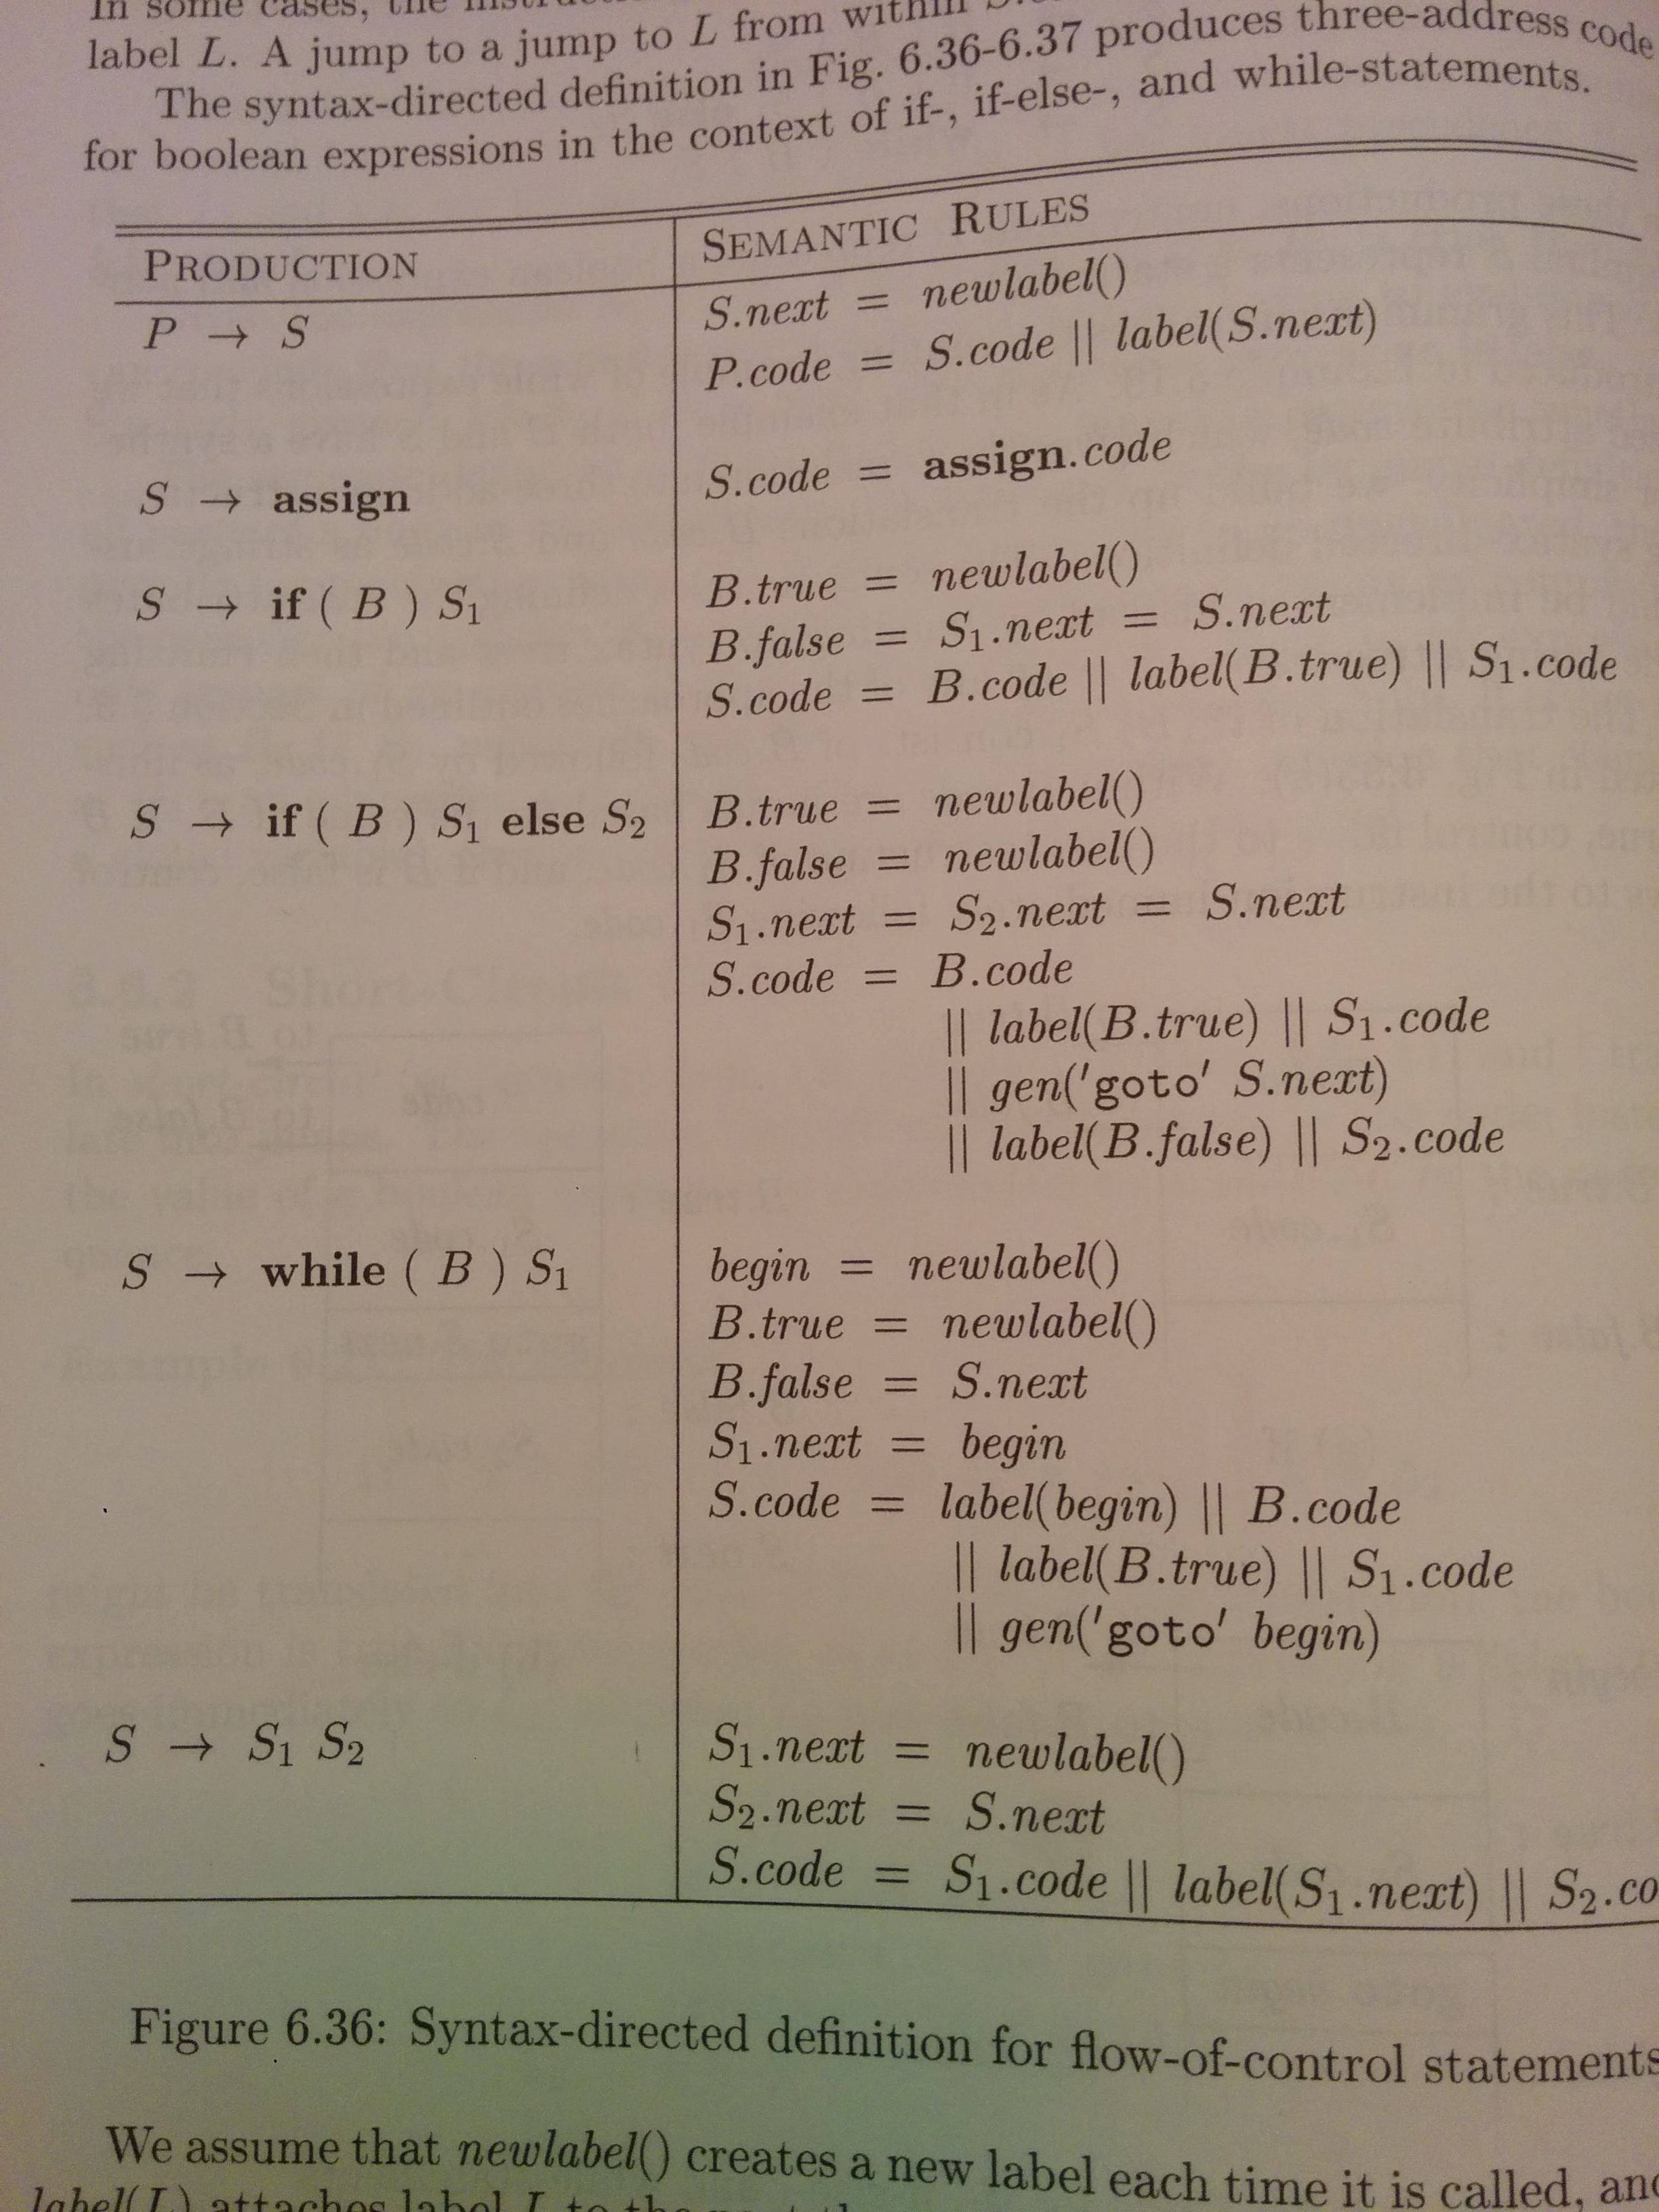
\includegraphics[scale=0.15]{IMG_20141029_013718.jpg} \\
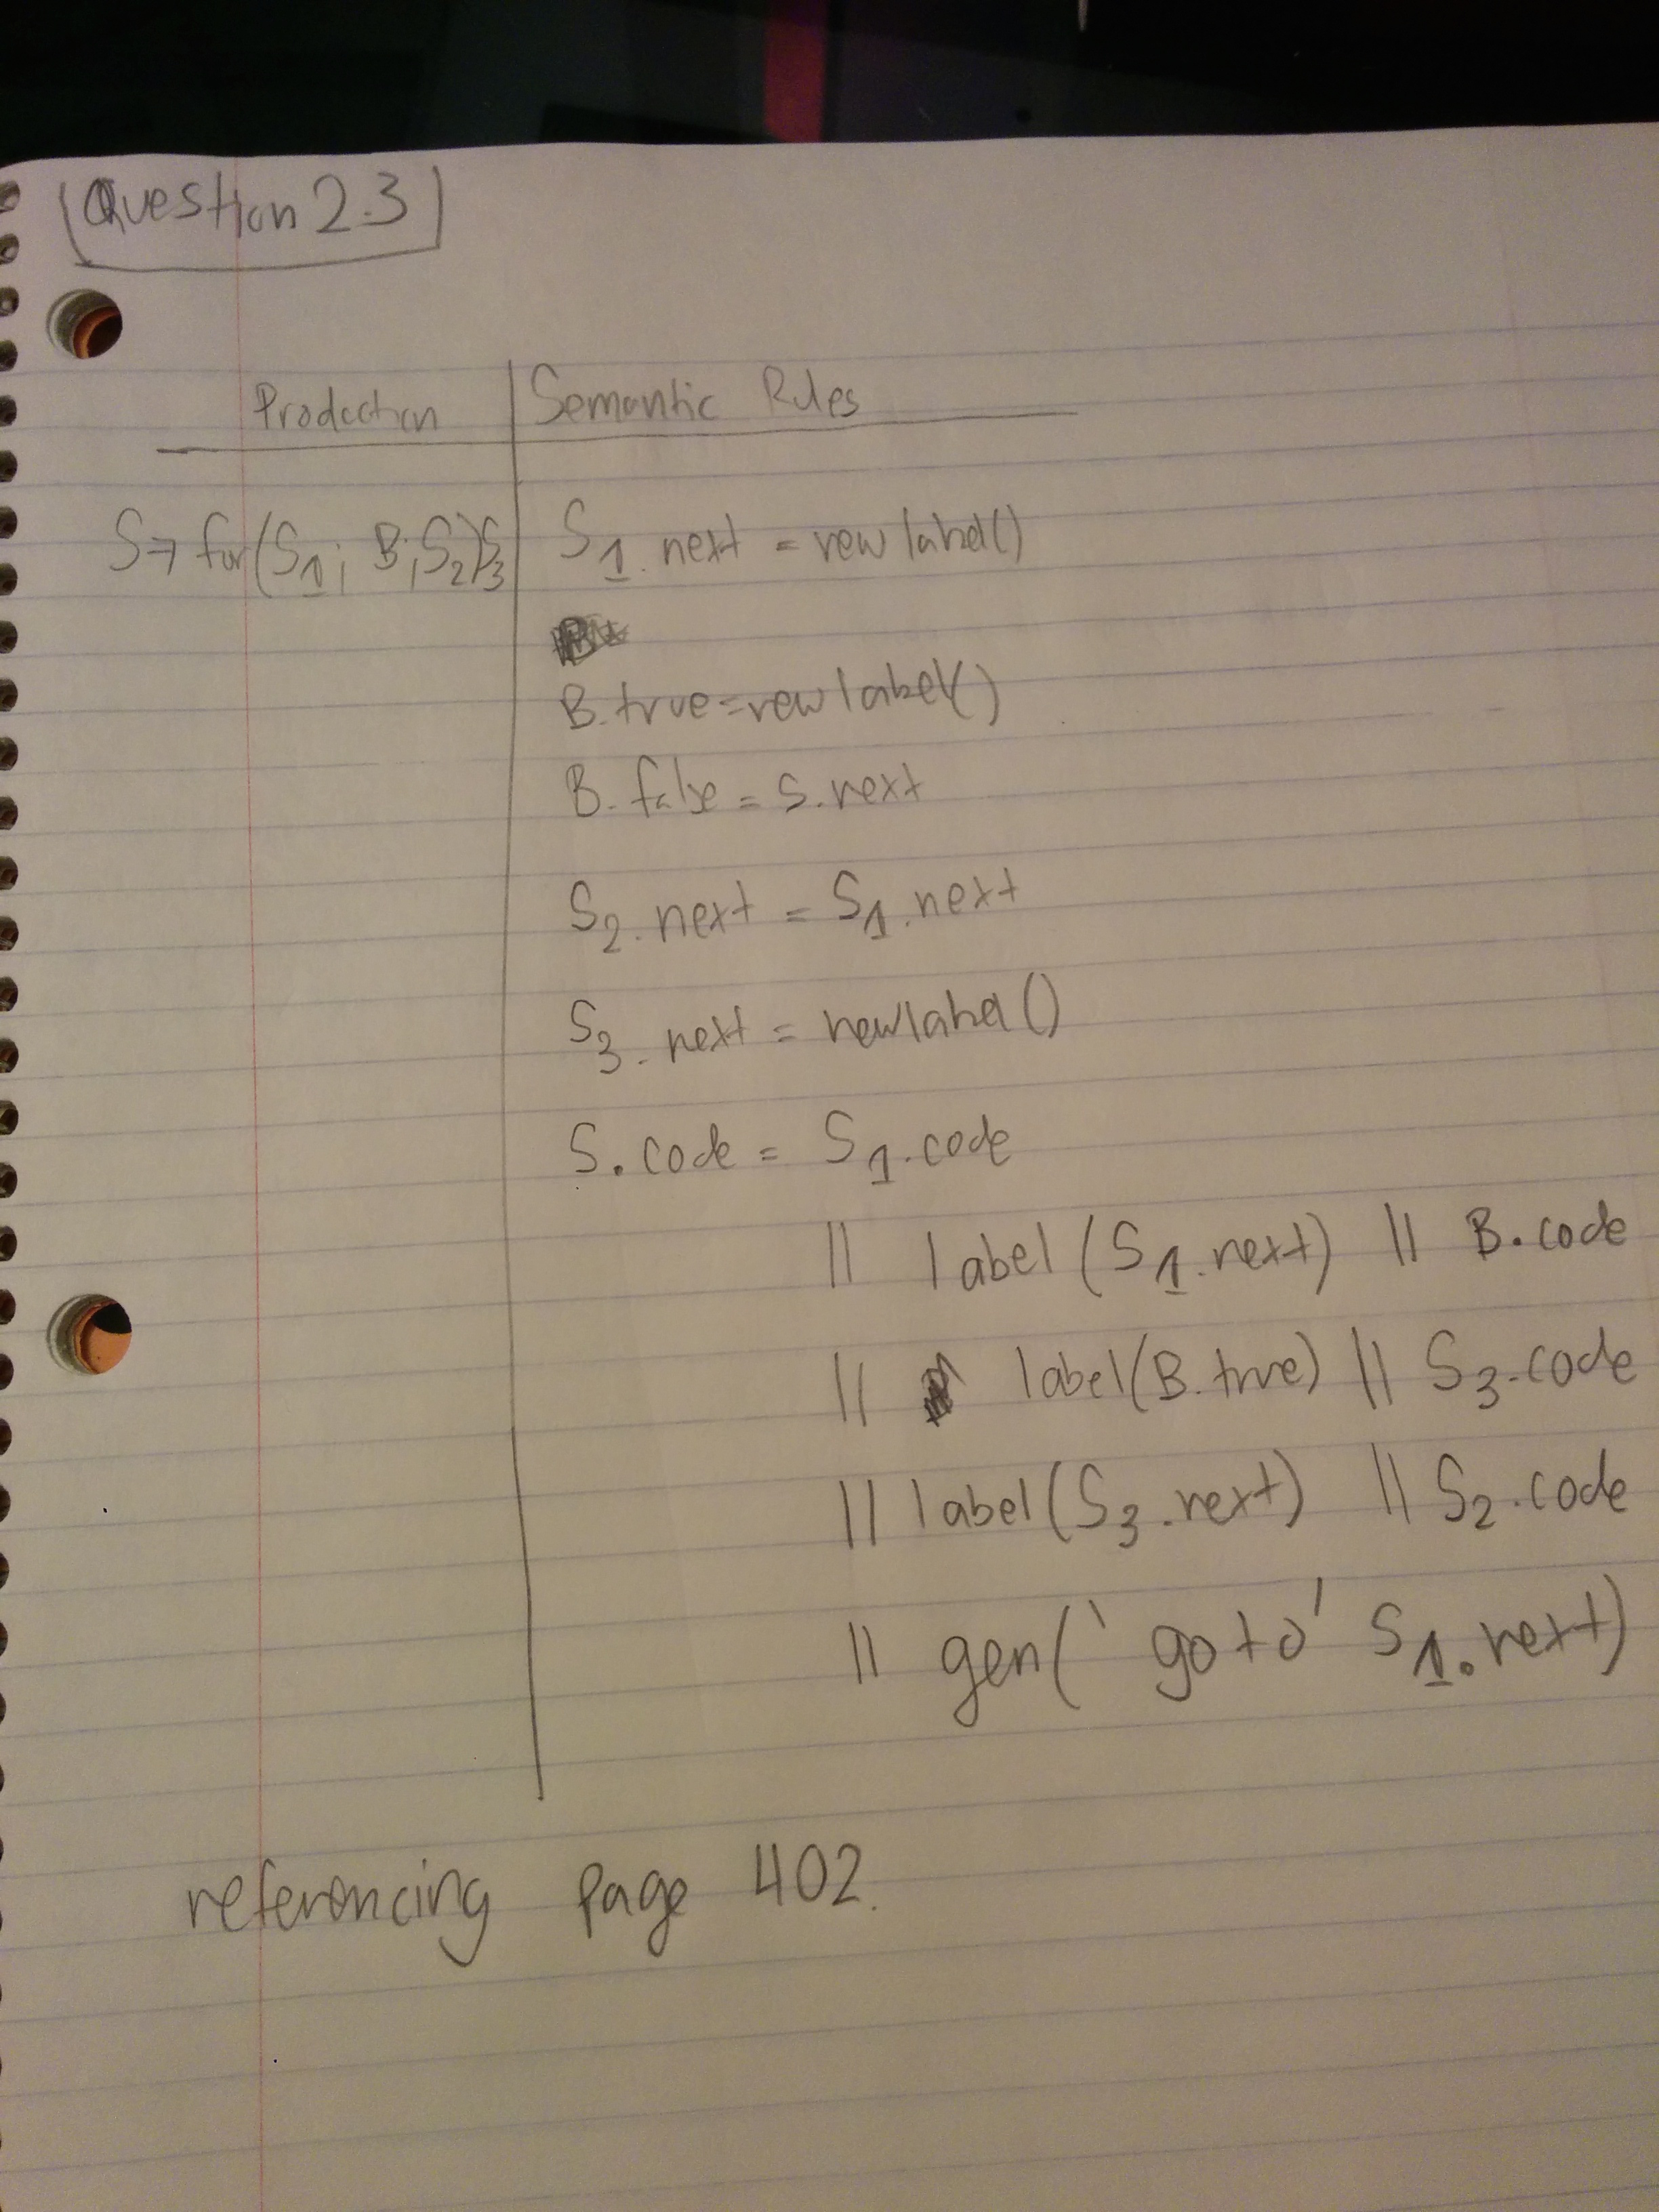
\includegraphics[scale=0.15]{IMG_20141029_014044.jpg}

\end{document}  